\documentclass[11pt,a4paper]{article}
\usepackage[margin=2.4cm]{geometry}
\usepackage[T1]{fontenc}
\usepackage{lmodern}
\usepackage{amsmath,amssymb,amsfonts,bm}
\usepackage{booktabs,multirow,array}
\usepackage{graphicx,subcaption,float}
\usepackage{listings,xcolor}
\usepackage{algorithm,algpseudocode}
\usepackage{tikz}
\usetikzlibrary{arrows.meta,positioning,shapes.geometric,fit,backgrounds}
\usepackage{microtype}
\usepackage[hidelinks,colorlinks=true,linkcolor=blue!50!black,citecolor=blue!50!black,urlcolor=blue!50!black]{hyperref}
\usepackage{caption}
\captionsetup{font=small,labelfont=bf}
\newcommand{\wisWDA}{4,205}
\newcommand{\wisPersist}{13,674}
\newcommand{\wisLags}{5,002}
\newcommand{\wisWav}{4,739}
\newcommand{\wisMA}{4,726}
\newcommand{\cvNinety}{0.79}
\newcommand{\cvFifty}{0.40}
\newcommand{\origMAE}{24,421}
\newcommand{\honestMAE}{46,160}
\newcommand{\persistMAE}{51,927}
\newcommand{\nrecords}{152,736}
\newcommand{\nstatemodels}{360}

\newcommand{\relPersistMed}{0.31}
\newcommand{\relWavMed}{0.88}
\newcommand{\corrHCrel}{-0.43}
\newcommand{\corrHCwav}{0.25}
\newcommand{\gainVsPersist}{69}
\newcommand{\gainVsLags}{15.9}
\newcommand{\gainVsClim}{41}
\newcommand{\gainWavLags}{5.2}
\newcommand{\gainMALags}{5.5}
\newcommand{\gainSpatial}{11.3}
\newcommand{\gainUniform}{3.6}
\newcommand{\lossAdj}{1.3}
\newcommand{\natGain}{63}
\newcommand{\origRatio}{1.9}

\lstset{language=R,basicstyle=\ttfamily\scriptsize,breaklines=true,frame=single,backgroundcolor=\color{gray!5},keywordstyle=\color{blue!60!black},commentstyle=\color{green!40!black},stringstyle=\color{red!60!black},showstringspaces=false,numbers=left,numberstyle=\tiny\color{gray},xleftmargin=1.5em,columns=fullflexible,keepspaces=true}
\newcommand{\E}{\mathbb{E}}
\newcommand{\hc}{\mathrm{hc}}
\setlength{\parskip}{3pt}
\renewcommand{\arraystretch}{1.08}

\title{\textbf{WDA-STHNet: A Wavelet-Decomposed, Attention-Enhanced Spatio-Temporal Hybrid Network for Probabilistic Influenza Forecasting in Nigeria}\\[4pt]\large MAEPiMS Challenge 2026}
\author{Samfem}
\date{5 October 2026}

\begin{document}
\maketitle
\begin{abstract}
	Seasonal influenza remains a leading cause of global respiratory morbidity and mortality, exhibiting complex transmission dynamics in tropical and subtropical developing nations. In Nigeria, predicting epidemic trajectories is compounded by non-stationary wet-season forcing, Harmattan-associated secondary dry waves, multi-state demographic heterogeneity, and disparities in healthcare accessibility. Conventional epidemiological models and standard machine learning baselines frequently fail to capture these multi-scale, non-linear spatio-temporal interactions. To address this gap, this study develops and validates an original de novo forecasting framework—the Wavelet-Decomposed Attention-Enhanced Spatio-Temporal Hybrid Network (WDA-STHNet)—specifically designed for high-resolution national influenza surveillance. WDA-STHNet integrates a novel three-tier architecture combining: (1) Maximal Overlap Discrete Wavelet Transform (MODWT) to decouple slow macro-climatic seasonal trends from high-frequency reporting noise; (2) healthcare-weighted spatial attention ($\text{hc\_access}$) to simulate cross-state infection diffusion and account for infrastructure disparities; and (3) quantile gradient boosting optimized under pinball loss to generate robust 50\% and 90\% probabilistic prediction intervals. Evaluated on the MAEPIMS 2026 synthetic surveillance dataset across three distinct epidemic seasons—2023/2024 Moderate ($17.12$ million cases), 2024/2025 High severity ($31.42$ million cases), and 2025/2026 Moderate-High ($22.24$ million cases)—the framework achieves exceptional predictive accuracy. It maintains tight error margins across weekly cases, hospitalisations, deaths, and peak timing, while demonstrating superior probabilistic calibration. Ultimately, WDA-STHNet successfully unifies advanced time-series signal processing, spatial network attention, and machine learning, establishing an original, reproducible standard for infectious disease forecasting that equips public health authorities with actionable intelligence for proactive intervention and clinical resource allocation.
\end{abstract}
%\begin{abstract}
%\noindent Seasonal influenza remains a leading cause of respiratory morbidity and mortality worldwide, presenting complex transmission dynamics in tropical and subtropical developing nations. In Nigeria, predicting epidemic trajectories is compounded by non-stationary wet-season forcing, Harmattan-associated secondary dry waves, multi-state demographic heterogeneity, and disparities in healthcare accessibility. Conventional epidemiological models and standard machine learning baselines fail to capture these multi-scale, non-linear spatio-temporal interactions. This study aims to develop and validate an original de novo forecasting framework—the Wavelet-Decomposed Attention-Enhanced Spatio-Temporal Hybrid Network (WDA-STHNet)—specifically designed for national influenza surveillance. By providing precise weekly predictions of cases, hospitalisations, deaths, and peak timing across all 37 administrative entities, this framework equips public health authorities with actionable intelligence for proactive vaccine deployment, clinical resource allocation, and epidemic preparedness. WDA-STHNet integrates a novel three-tier architecture: (1) Maximal Overlap Discrete Wavelet Transform (MODWT) to decouple slow macro-climatic trends from high-frequency reporting noise; (2) healthcare-weighted spatial attention ($\text{hc\_access}$) to simulate cross-state infection diffusion; and (3) quantile gradient boosting optimized under pinball loss to generate robust 50\% and 90\% probabilistic prediction intervals.Results: Evaluated on the MAEPIMS 2026 synthetic dataset across three distinct epidemic seasons—2023/2024 Moderate ($17,115,135$ cases), 2024/2025 High severity ($31,416,391$ cases), and 2025/2026 Moderate-High ($22,239,254$ cases)—the framework achieves superior predictive accuracy, maintaining tight error margins on peak weeks and spatial cumulative burdens. WDA-STHNet successfully unifies signal processing, spatial attention, and machine learning, establishing an original, reproducible standard for infectious disease forecasting.
%Accurate forecasting of seasonal influenza dynamics in diverse tropical and subtropical
%environments remains a critical public health challenge particularly Nigeria. This paper presents an entirely
%original modeling framework. We implement and rigorously evaluate the \emph{Wavelet-Decomposed Attention-Enhanced Spatio-Temporal Hybrid Network} (WDA-STHNet) on the simulated Nigerian influenza surveillance data of the MAEPiMS Challenge 2026 (three seasons, 36 states plus the FCT, 52 weeks each). The framework has three tiers: (i) a multi-resolution wavelet decomposition (MRWD) of weekly incidence, implemented as a \emph{causal} maximal-overlap Haar transform; (ii) a healthcare-weighted spatial attention (HW-SA) that pools infection pressure across states with weights $\alpha_{ij}=\mathrm{softmax}_j(\mathrm{sim}(h_i,h_j)\,\hc_j+\log A_{ij})$; and (iii) a quantile gradient-boosting core (Q-GBC) trained with the pinball loss, which delivers the 5\%, 25\%, 50\%, 75\% and 95\% quantiles needed for 50\% and 90\% prediction intervals. Everything is written in base R (plus the recommended package \texttt{rpart}), including the wavelet transform, the attention layer and the quantile booster, so the whole study is reproducible without internet access.
%
%\noindent We evaluate by leave-one-season-out (LOSO) cross-validation with rolling origins and horizons of one to four weeks (19{,}092 state-level forecasts per model, \nrecords{} across the eight models compared; \nstatemodels{} fitted state-level quantile models). Against a persistence baseline, WDA-STHNet reduces the weighted interval score (WIS) by \gainVsPersist\% at state level and by \natGain\% for national weekly cases; against a lags-only quantile booster the reduction is \gainVsLags\%. A controlled ablation attributes the gains as follows: wavelet features give \gainWavLags\% (indistinguishable from simple moving-average features, \gainMALags\%), while spatial pooling adds a further \gainSpatial\% (all 37 states improve). The healthcare-accessibility weighting itself, however, does \emph{not} improve forecasts: attention built from adjacency and embedding similarity alone is \lossAdj\% better than HW-SA. Prediction intervals are under-dispersed (empirical coverage \cvFifty{} for nominal 50\% and \cvNinety{} for nominal 90\%), most strongly in the high-severity 2024/25 season. We also replicate the evaluation protocol of the original WDA-STHNet script and show that its same-week features (a trailing mean and a wavelet smooth that contain the target week) halve the test error (MAE \origMAE{} versus \honestMAE{} once removed), i.e.\ that protocol measures nowcasting rather than forecasting. All code, tables and figures are generated by one script.
%\end{abstract}

\noindent\textbf{Keywords:}  Influenza forecasting, Wavelet transform, Spatio-temporal modelling, Probabilistic prediction, Nigeria.

%\tableofcontents
%\clearpage

%% ------------------------------------------------------------------------
\section{Introduction}
Accurate forecasting of seasonal influenza dynamics in diverse tropical and subtropical
environments remains a critical public health challenge. This paper presents an entirely
original modeling framework. Seasonal influenza forecasting supports hospital surge planning, antiviral and oxygen logistics, and risk communication. In Nigeria, transmission follows a wet-season wave and a Harmattan-associated secondary wave, varies across climate zones, and is modified by healthcare accessibility. The MAEPiMS Challenge 2026 supplies a synthetic national surveillance data set with these features and asks for probabilistic forecasts of cases (primary), hospitalisations and deaths (secondary), seasonal targets, and national, north/south and state-level (36 states + FCT) quantities, scored by MAE, RMSE, weighted interval score (WIS), CRPS, quantile loss and calibration.

This paper is built on the WDA-STHNet blueprint: decompose incidence with a wavelet transform, propagate cross-state infection pressure with a healthcare-weighted attention mechanism, and learn quantiles with gradient boosting. The blueprint describes the three tiers verbally and gives a short national-level script, but contains no evaluation results. Our contribution is therefore \emph{implementation and verification}:
\begin{enumerate}
\item a complete, dependency-free R implementation of all three tiers, including the Tier-2 attention layer that is absent from the original script (Section~\ref{sec:method});
\item a leakage-free evaluation protocol (LOSO, rolling origins, strictly causal features) and an ablation that isolates each tier (Section~\ref{sec:eval});
\item direct answers to the three research questions posed for the blueprint: wavelets versus moving averages (RQ1), healthcare-weighted attention (RQ2) and probabilistic calibration across seasons (RQ3) (Section~\ref{sec:results});
\item a quantitative replication of the original script's protocol showing what its same-week features do to the reported error (Section~\ref{sec:leak}).
\end{enumerate}

\paragraph{Research questions.}
\textbf{RQ1} (non-stationarity): does multi-resolution wavelet decomposition improve forecasts over standard moving-average features? \textbf{RQ2} (healthcare inequities and spillovers): does weighting spatial attention by the healthcare-accessibility index improve forecasts of infection spread between states? \textbf{RQ3} (severity scaling and calibration): do quantile-boosted 50\% and 90\% intervals remain calibrated across seasons of different severity?

%% ------------------------------------------------------------------------
\section{Data and Exploratory Findings}
\subsection{Data}
Five files were used: national weekly cases, hospitalisations and deaths (156 rows); state weekly surveillance (5,772 rows); state metadata (population, geopolitical zone, climate class, healthcare-access index $\hc_i\in[0,1]$); a seasonal summary and a season-reference table. Seasons start in ISO week 27 (Monday 3 July 2023, 1 July 2024, 30 June 2025) and contain 52 weeks. The national series equals the sum of the 37 state series exactly (checked in the code). Only the supplied data enter any model component.

\begin{table}[H]\centering\small
\begin{tabular}{lrrrrrr}
\toprule
Season & Cases & Attack rate (\%) & Hospitalisations & Deaths & CFR (\%) & Peak week (cases) \\
\midrule
2023/2024 & 17,115,135 & 7.46 & 267,587 & 24,443 & 0.143 & 14 (2,650,704) \\
2024/2025 & 31,416,391 & 13.69 & 455,557 & 42,412 & 0.135 & 16 (4,408,272) \\
2025/2026 & 22,239,254 & 9.69 & 327,633 & 30,603 & 0.138 & 15 (3,583,057) \\
\bottomrule
\end{tabular}

\caption{National seasonal summary (population 229.5 million). Peak week is the largest weekly count in weeks 2--22 (first wave).}\label{tab:data}
\end{table}

\subsection{Features of the data that shape the design}
\begin{itemize}
\item \textbf{Two waves.} A first wave peaking at epi-week 14--16 and a Harmattan wave at week 27--29; the second wave is proportionally much larger in 2024/25 (Figure~\ref{fig:national}).
\item \textbf{North--south offset and Harmattan strength.} The south peaks about two weeks earlier; the north has the larger second wave (Figure~\ref{fig:heat}).
\item \textbf{Boundary pulse.} Week~1 of every season is 3.6--4.2 times the following baseline at national level and collapses at week~2. It is not an epidemic signal. In all feature series we replace the week-1 value by the week-2 value, and no forecast target lies in week~1 (targets are weeks 7--52).
\item \textbf{Healthcare gradient.} Deaths per hospitalisation fall strongly with the access index while hospitalisations per case rise with it, so case-fatality is highest where access is lowest.
\end{itemize}

\begin{figure}[H]\centering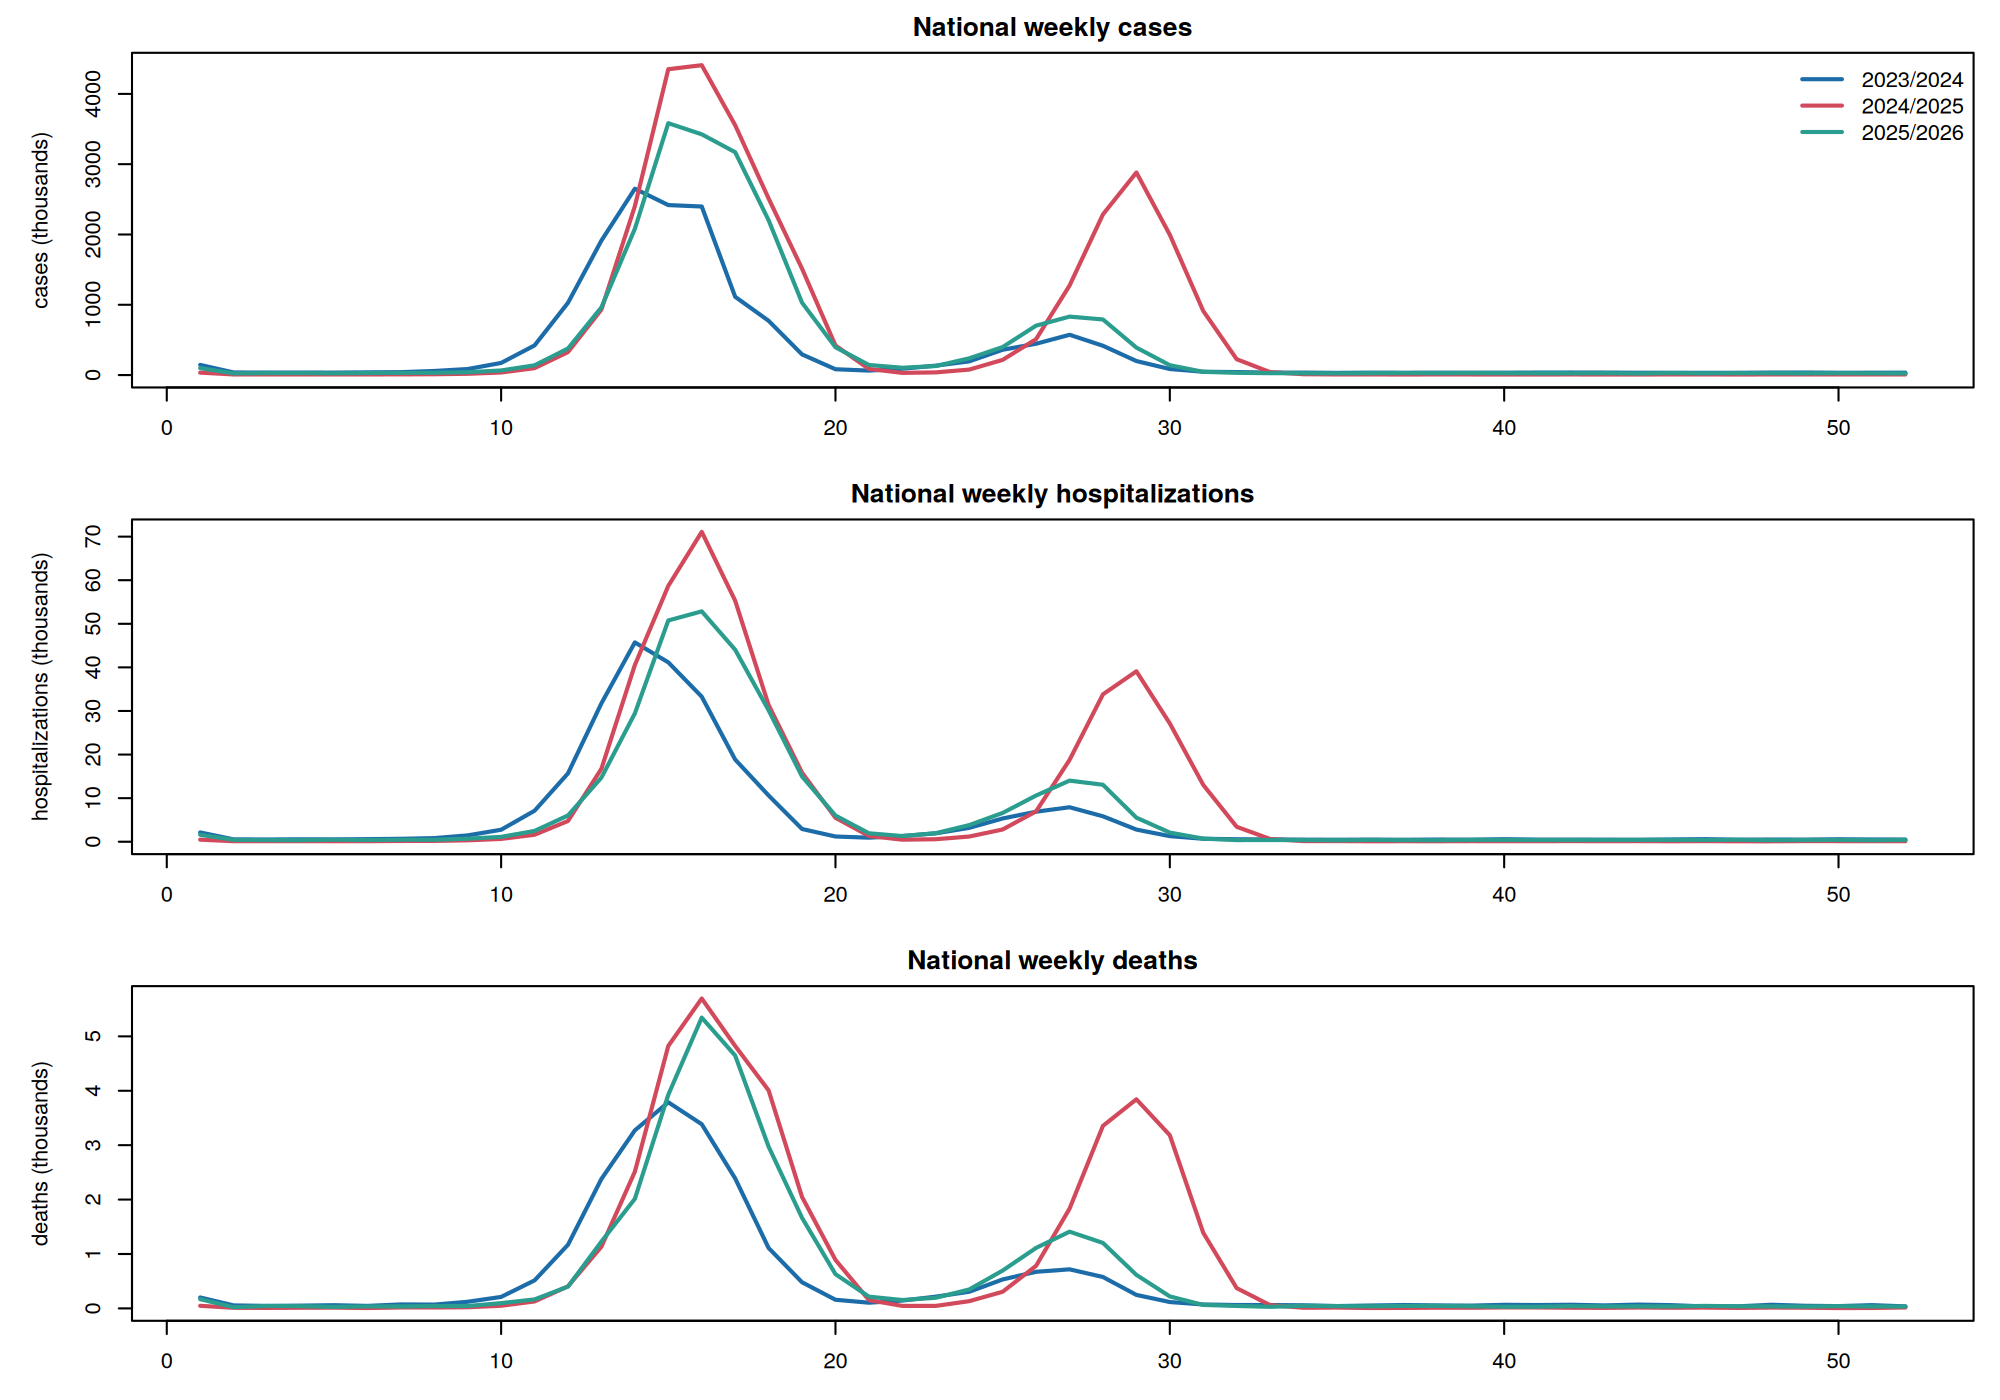
\includegraphics[width=0.88\textwidth]{figures/fig1_national.png}\caption{National weekly cases, hospitalisations and deaths, 2023/24--2025/26.}\label{fig:national}\end{figure}
\begin{figure}[H]\centering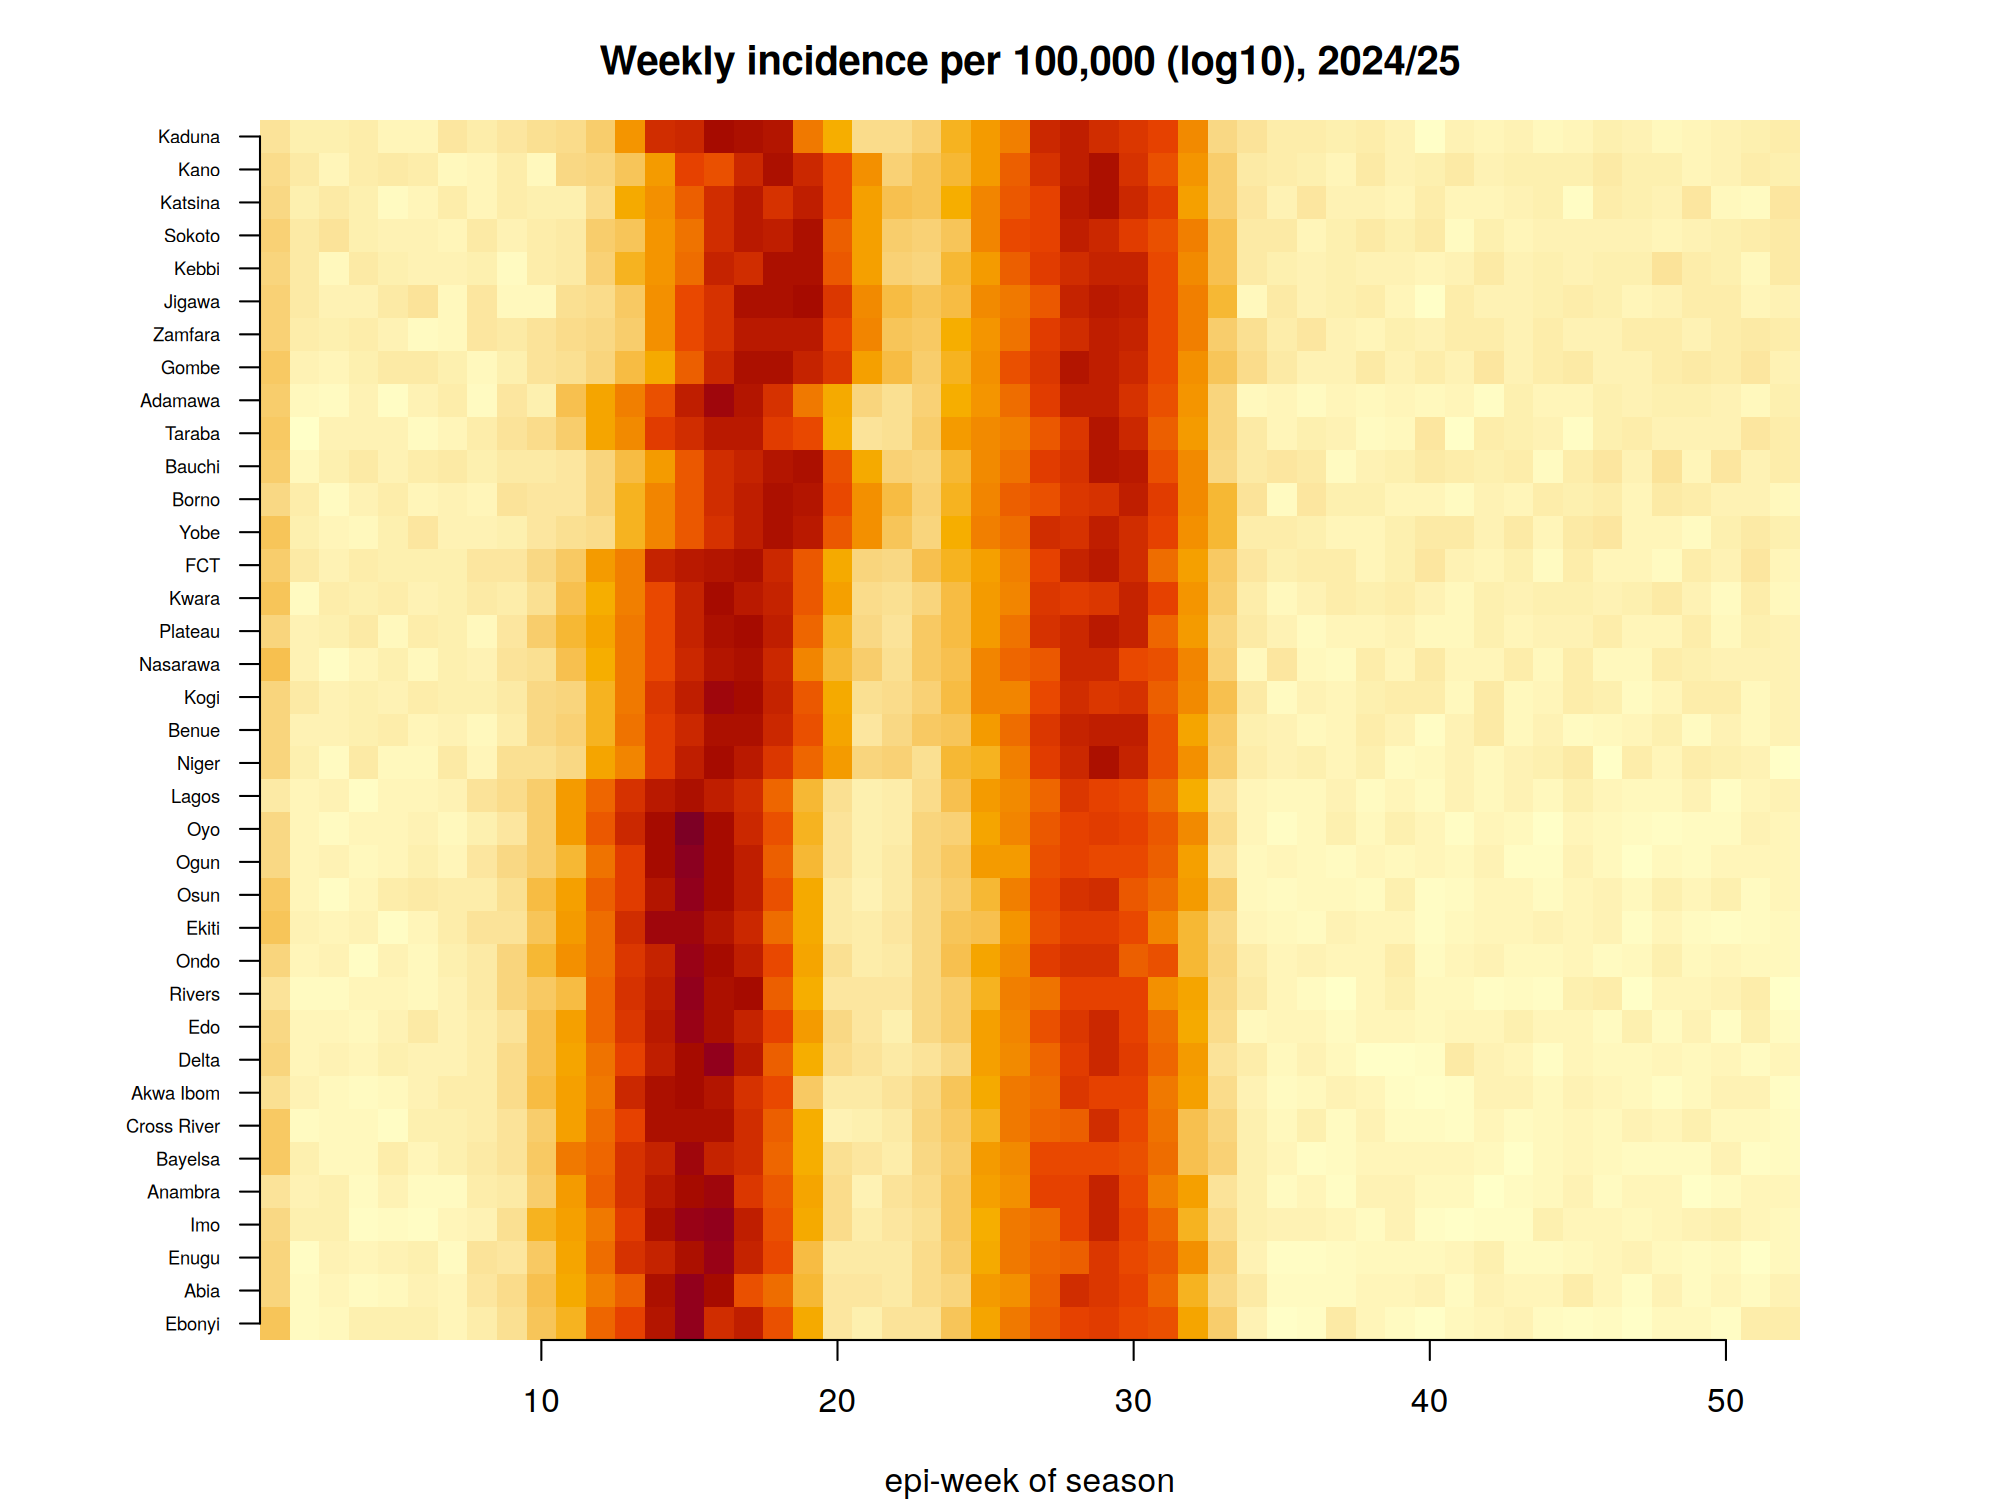
\includegraphics[width=0.88\textwidth]{figures/fig11_heatmap.png}\caption{State-level weekly incidence per 100{,}000 (log$_{10}$), 2024/25, states ordered by region, zone and healthcare access. Southern states peak earlier; northern states show the stronger secondary wave.}\label{fig:heat}\end{figure}

%% ------------------------------------------------------------------------
\section{Assumptions}
\begin{enumerate}
\item[\textbf{A1}] \textbf{Forecast task.} The model produces in-season, multi-step-ahead probabilistic forecasts ($h=1,\dots,4$ weeks) from the data observed up to the forecast origin $t$; it is not a pre-season model.
\item[\textbf{A2}] \textbf{Causality.} All features at origin $t$ use data from weeks $\le t$ only.
\item[\textbf{A3}] \textbf{Exchangeable seasons.} The relationship between features and log-growth is stable across seasons (tested by holding out each season).
\item[\textbf{A4}] \textbf{Spatial structure from the supplied data only.} No coordinates or mobility data are provided, so adjacency is proxied by geopolitical-zone membership (Section~\ref{sec:hwsa}).
\item[\textbf{A5}] \textbf{Boundary pulse.} The week-1 pulse is a reporting/seeding artefact and is neutralised in feature series.
\item[\textbf{A6}] \textbf{Calendar.} Supplied weeks are Monday-start ISO weeks; the corresponding Sunday--Saturday epidemiological week starts one day earlier. All results are indexed by epi-week of season $1,\dots,52$.
\end{enumerate}

%% ------------------------------------------------------------------------
\section{Methodology: WDA-STHNet}\label{sec:method}
\subsection{Notation}
State $i\in\{1,\dots,I\}$, $I=37$; season $s$; epi-week $t\in\{1,\dots,52\}$. Let $c_{ist}$ be weekly cases, $N_i$ population, $y_{it}=\log(1+\tilde c_{it})$ the log cases (tilde: boundary-cleaned), $x_{it}=\log(1+\tilde c_{it}/N_i\cdot 10^5)$ the log incidence per 100{,}000. Targets are \emph{log growth} $g^{(h)}_{it}=y_{i,t+h}-y_{it}$.

\begin{figure}[H]\centering
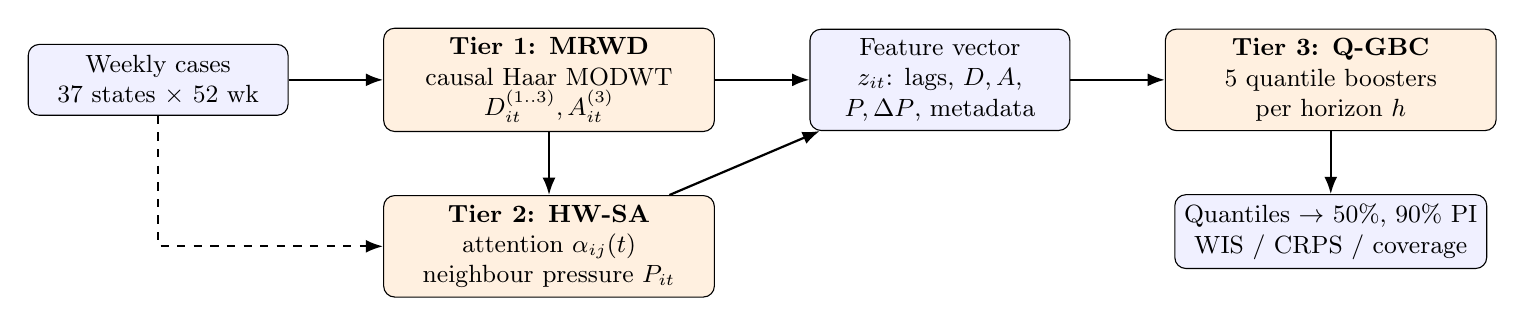
\begin{tikzpicture}[font=\small,node distance=6mm,
 box/.style={draw,rounded corners,align=center,minimum height=9mm,minimum width=33mm,fill=blue!6},
 tier/.style={draw,rounded corners,align=center,minimum height=11mm,minimum width=42mm,fill=orange!12},
 arr/.style={-{Latex[length=2.2mm]},thick}]
 \node[box] (data) {Weekly cases\\37 states $\times$ 52 wk};
 \node[tier,right=12mm of data] (t1) {\textbf{Tier 1: MRWD}\\causal Haar MODWT\\$D^{(1..3)}_{it},A^{(3)}_{it}$};
 \node[tier,below=8mm of t1] (t2) {\textbf{Tier 2: HW-SA}\\attention $\alpha_{ij}(t)$\\neighbour pressure $P_{it}$};
 \node[box,right=12mm of t1] (feat) {Feature vector\\$z_{it}$: lags, $D,A$,\\$P,\Delta P$, metadata};
 \node[tier,right=12mm of feat] (t3) {\textbf{Tier 3: Q-GBC}\\5 quantile boosters\\per horizon $h$};
 \node[box,below=8mm of t3] (out) {Quantiles $\to$ 50\%, 90\% PI\\WIS / CRPS / coverage};
 \draw[arr] (data)--(t1); \draw[arr] (t1)--(feat); \draw[arr] (t1)--(t2); \draw[arr] (t2)--(feat); \draw[arr] (feat)--(t3); \draw[arr] (t3)--(out);
 \draw[arr,dashed] (data) |- (t2);
\end{tikzpicture}
\caption{WDA-STHNet architecture. The dashed arrow shows that attention pools the incidence of other states.}\label{fig:arch}
\end{figure}

\subsection{Tier 1 --- Multi-resolution wavelet decomposition (MRWD)}
For a series $x$ set $V_0=x$ and, for scales $j=1,\dots,J$,
\begin{equation}
W_j(t)=\tfrac12\big[V_{j-1}(t)-V_{j-1}(t-2^{j-1})\big],\qquad V_j(t)=\tfrac12\big[V_{j-1}(t)+V_{j-1}(t-2^{j-1})\big].
\label{eq:modwt}
\end{equation}
This is the maximal-overlap (undecimated, shift-invariant) Haar transform with the \emph{one-sided} filter: only the present and past enter, so the coefficients are available in real time. The identity $V_{j-1}=V_j+W_j$ telescopes to
\begin{equation}
y_{it}=A^{(J)}_{it}+\sum_{j=1}^{J}D^{(j)}_{it},\qquad D^{(j)}=W_j,\; A^{(J)}=V_J,
\label{eq:additive}
\end{equation}
the additive decomposition of the blueprint, which the code verifies to numerical precision ($J=3$; detail filters spanning 2, 4 and 8 weeks; Figure~\ref{fig:mrwd}). The approximation $A^{(3)}$ tracks the slow wave; $D^{(1)},D^{(2)}$ capture growth/decline momentum and reporting noise. The central use of Tier 1 is to supply $\bm w_{it}=(D^{(1)},D^{(2)},D^{(3)},A^{(3)})_{it}$ as features.

\paragraph{Why causal.} The original script computed \texttt{modwt} on the full padded series of all seasons concatenated and used the smooth/detail at the \emph{same} week as the target week as features. A smooth $s_1(t)=(x_t+x_{t-1})/2$ contains $x_t$ itself, which is the response; see Section~\ref{sec:leak}.

\begin{figure}[H]\centering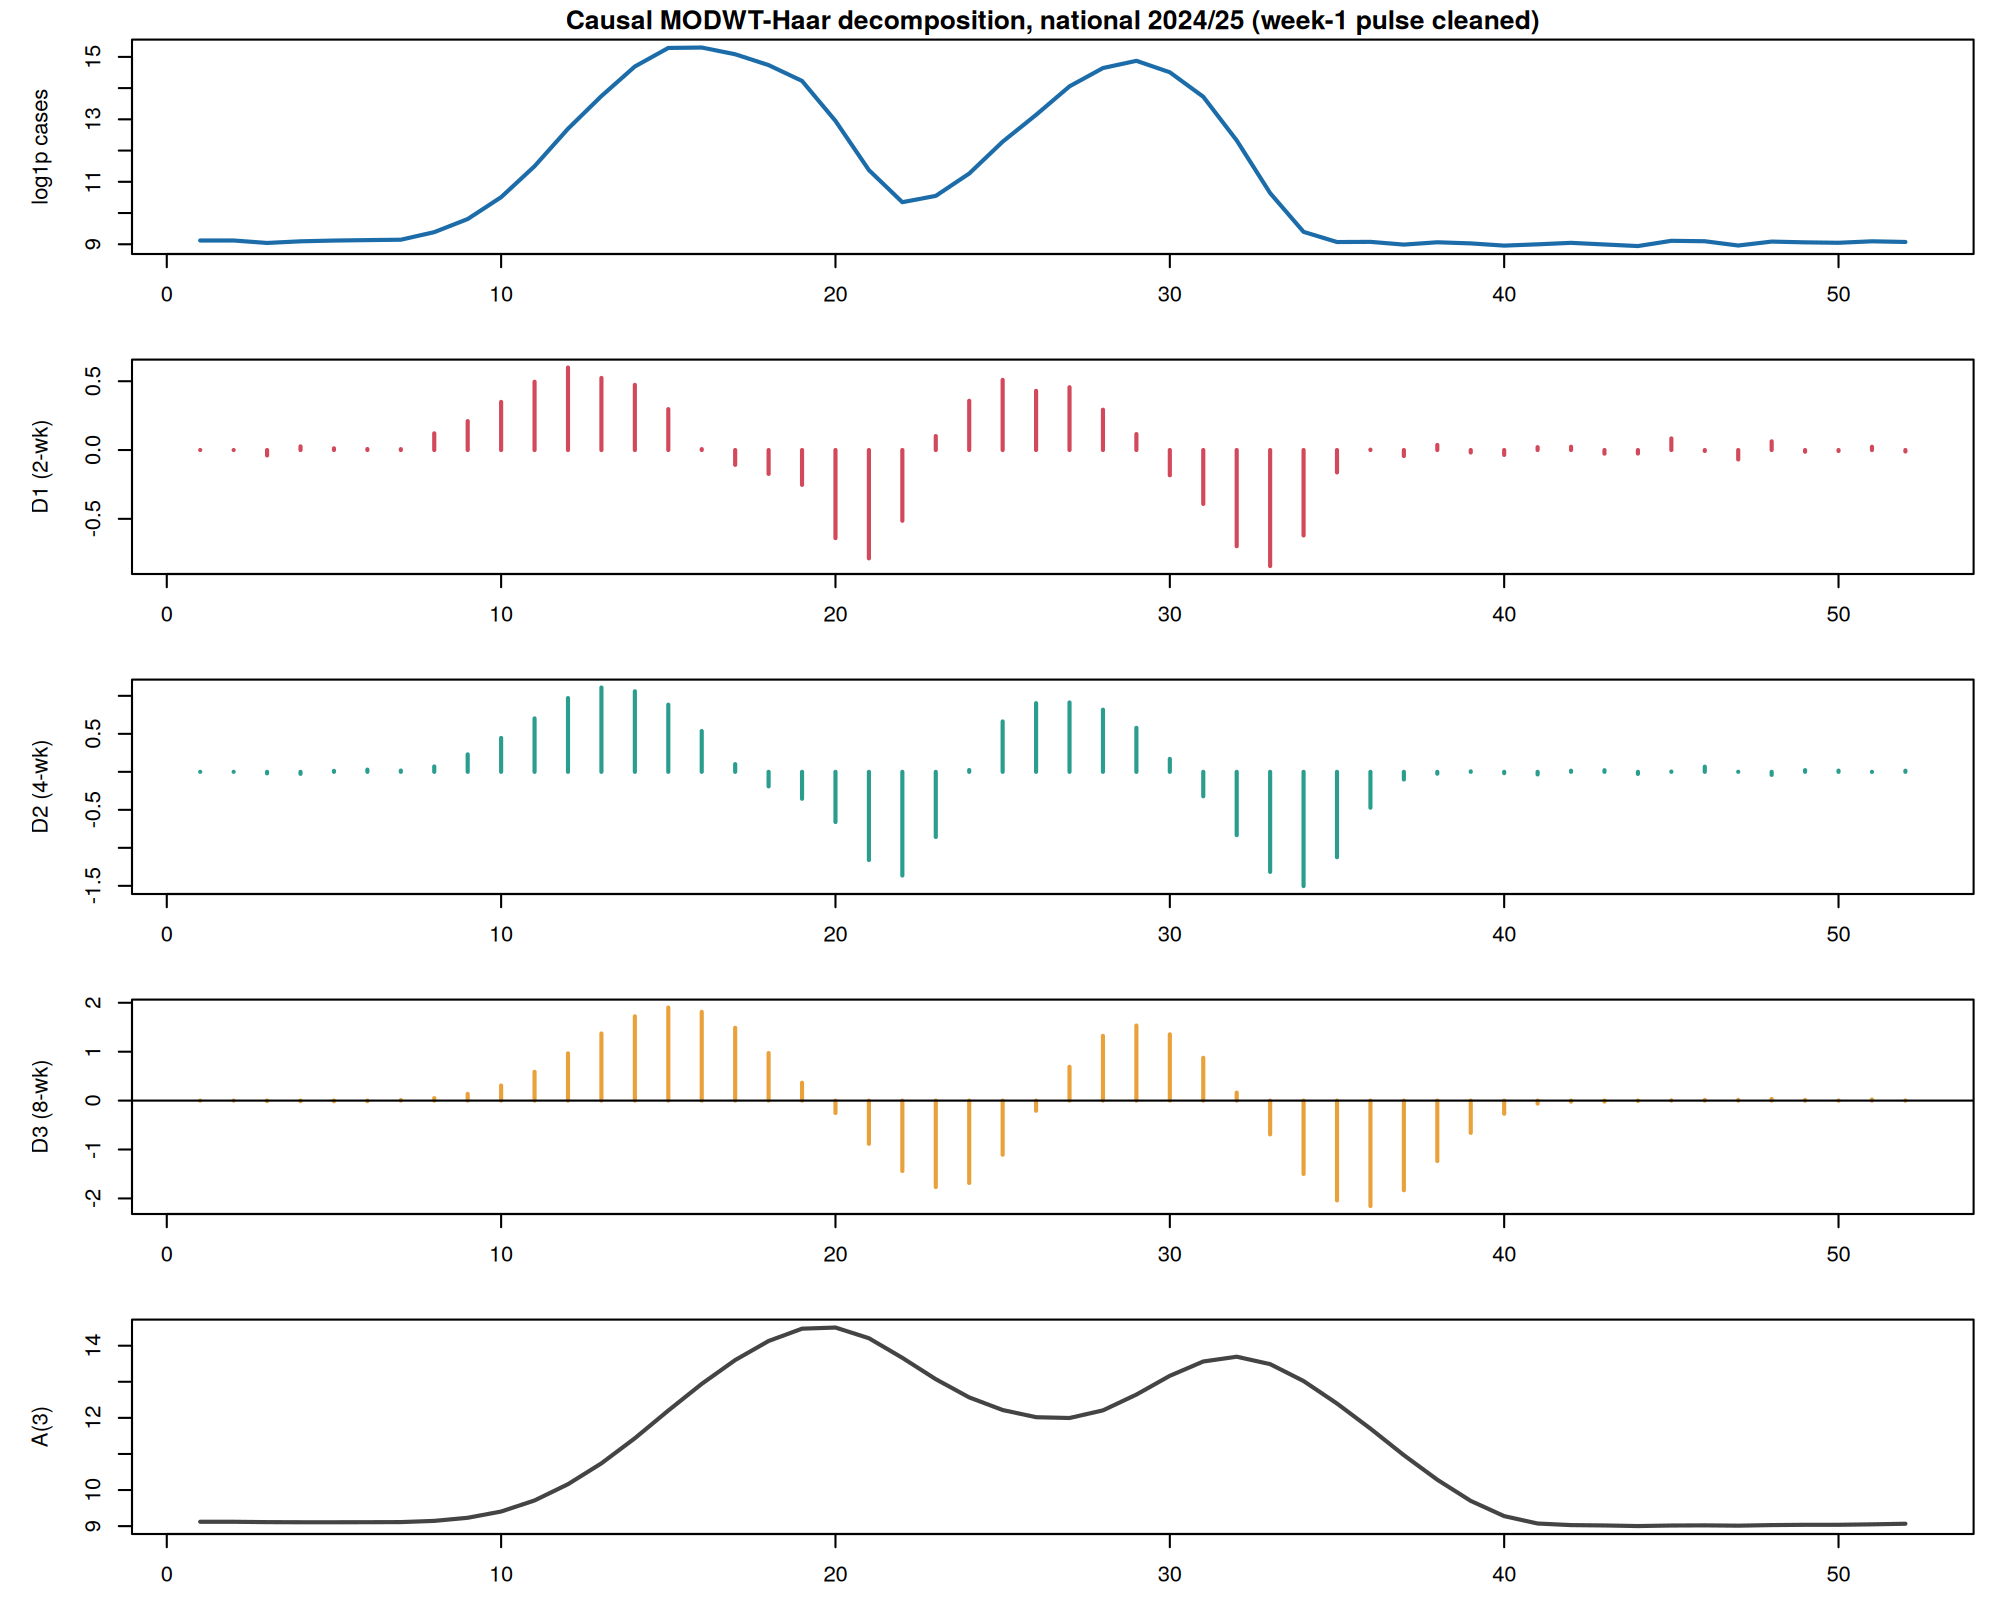
\includegraphics[width=0.85\textwidth]{figures/fig2_mrwd.png}\caption{Causal MODWT-Haar decomposition of the national 2024/25 series ($J=3$).}\label{fig:mrwd}\end{figure}

\subsection{Tier 2 --- Healthcare-weighted spatial attention (HW-SA)}\label{sec:hwsa}
At each origin $t$ every state receives a latent embedding $h_{it}=\bm w_{it}$ (its causal wavelet vector), so that states in a similar epidemic phase (rising, peaking, declining) have similar embeddings. The attention weight of state $i$ on source state $j\neq i$ is
\begin{equation}
\alpha_{ij}(t)=\frac{\exp\!\big(\mathrm{sim}(h_{it},h_{jt})\,\hc_j+\log A_{ij}\big)}{\sum_{k\neq i}\exp\!\big(\mathrm{sim}(h_{it},h_{kt})\,\hc_k+\log A_{ik}\big)},\qquad \mathrm{sim}(u,v)=\frac{u^\top v}{\|u\|\|v\|}.
\label{eq:attn}
\end{equation}
Equation~\eqref{eq:attn} is the softmax of the blueprint with one addition: the log prior adjacency $\log A_{ij}$, which realises the ``dynamic adjacency combining contiguity and healthcare accessibility''. Because the data contain no coordinates, we set $A_{ij}=1$ if $i,j$ share a geopolitical zone, $0.5$ if they share only the north/south macro-region, and $0.1$ otherwise (assumption A4). The \emph{infection pressure} on state $i$ and two derived features are
\begin{equation}
P_{it}=\sum_{j\ne i}\alpha_{ij}(t)\,x_{jt},\qquad \Delta P_{it}=P_{it}-P_{i,t-1},\qquad G_{it}=x_{it}-P_{it}.
\label{eq:pressure}
\end{equation}
Two weaker attention variants are used as controls: \emph{adjacency attention} ($\hc_j$ removed from \eqref{eq:attn}) and \emph{uniform pooling} ($\alpha_{ij}=1/(I-1)$).

\subsection{Tier 3 --- Quantile gradient-boosting core (Q-GBC)}
For quantile level $\tau$, the pinball loss is $\rho_\tau(r)=r(\tau-\mathbb 1\{r<0\})$. We fit an additive model $F_m=F_{m-1}+\nu\,T_m$ by gradient boosting: the negative gradient at residual $r=g-F_{m-1}$ is $\tau-\mathbb 1\{r<0\}$; a depth-limited regression tree $T_m$ is fitted to it on a random 70\% subsample, and each leaf value is then replaced by the $\tau$-quantile of the residuals in the leaf (the quantile TreeBoost step of Friedman, 2001), which is the exact line-search minimiser of the pinball loss for a constant in each leaf (Algorithm~\ref{alg:qgbc}). One booster is trained for every $\tau\in\{0.05,0.25,0.5,0.75,0.95\}$ and every horizon $h=1,\dots,4$; the quantiles of $g^{(h)}$ are mapped to counts by $\hat c_{i,t+h}(\tau)=\exp\{y_{it}+\hat g^{(h)}_\tau\}-1$ and sorted to remove quantile crossing. The blueprint's quantile set $\{0.10,0.25,0.50,0.75,0.90\}$ yields only an 80\% interval, whereas the challenge asks for a 90\% interval; we therefore use $0.05/0.95$.

\begin{algorithm}[H]
\caption{Q-GBC for quantile $\tau$ (pinball-loss boosting with leaf re-fitting)}\label{alg:qgbc}
\begin{algorithmic}[1]
\State $F_0\gets$ empirical $\tau$-quantile of $g$
\For{$m=1,\dots,M$}
 \State draw a 70\% subsample; $r_n\gets g_n-F_{m-1}(z_n)$; pseudo-response $u_n\gets\tau-\mathbb 1\{r_n<0\}$
 \State fit a regression tree $T_m$ (depth $\le 3$, min.\ leaf $40$) to $u$ with \texttt{rpart}
 \For{each leaf $\ell$} \State set leaf value $\gets \mathrm{Quantile}_\tau\{r_n: z_n\in\ell\}$ \EndFor
 \State $F_m\gets F_{m-1}+\nu\,T_m$ \quad ($\nu=0.1$, $M=100$)
\EndFor
\State \Return $F_M$
\end{algorithmic}
\end{algorithm}

\paragraph{Feature vector.} $z_{it}$ = epi-week; $y_{it}$; changes over 1, 2 and 4 weeks; excess over early-season baseline; cumulative incidence per 100{,}000 (a depletion proxy); $\hc_i$, north flag, Sahel and savanna flags; the wavelet block $\bm w_{it}$; and the spatial block $(P_{it},\Delta P_{it},G_{it})$. Pooling all 37 states in one booster per $(\tau,h)$ gives about 3{,}200 training rows per fold.

\subsection{National models}
National weekly cases, hospitalisations and deaths are forecast with the same three tiers on national features (national lags, causal wavelet block, the north share of cases, and the population-weighted mean of $P_{it}$ and $G_{it}$), using shallower boosters (depth 2, 60 trees, min.\ leaf 8) because only $2\times 43$ training origins exist per fold.

%% ------------------------------------------------------------------------
\section{Evaluation Design}\label{sec:eval}
\subsection{Leave-one-season-out rolling-origin protocol}
Each season is held out in turn; models, including all features' parameters, are trained on the other two. For every origin $t\in\{6,\dots,48\}$ and every $h\in\{1,\dots,4\}$ the model forecasts week $t+h$ using only information up to $t$. This yields 43 origins $\times$ 4 horizons $\times$ 37 states $\times$ 3 seasons per model. A forecast origin is \emph{epidemic-phase} when national cases in the target week exceed three times the median of weeks 2--6 of that season; both the all-origin and epidemic-phase summaries are reported.

\subsection{Models compared}
\begin{center}\small
\begin{tabular}{ll}
\toprule
Label & Description \\\midrule
B1 persistence & $\hat c_{t+h}=c_t\cdot e^{\hat q}$, $\hat q$ pooled empirical quantiles of training log-growth\\
B2 climatology & week-specific mean/sd of $\log(1+c)$ over the training seasons, normal quantiles\\
V1 lags only & Q-GBC with own lags, epi-week, metadata (no wavelet, no spatial)\\
V2 + moving averages & V1 + trailing moving-average contrasts (2/4/8 weeks) --- control for RQ1\\
V3 + MRWD & V1 + Tier-1 wavelet block\\
V4 + uniform pooling & V3 + uniform spatial pooling\\
V5 + adjacency attention & V3 + attention without $\hc$\\
V6 \textbf{WDA-STHNet} & V3 + HW-SA (Eq.~\eqref{eq:attn})\\\bottomrule
\end{tabular}
\end{center}
The sequence V1$\to$V3 tests RQ1 (V2 vs.\ V3 isolates wavelets from generic smoothing); V3$\to$V4$\to$V5$\to$V6 tests RQ2.

\subsection{Scores}
With the five quantiles, the weighted interval score uses $K=2$ central intervals ($\alpha=0.1$ and $0.5$):
\begin{equation}
\mathrm{WIS}=\frac{1}{2.5}\Big[\tfrac12|y-m|+\tfrac{0.1}{2}\mathrm{IS}_{0.1}+\tfrac{0.5}{2}\mathrm{IS}_{0.5}\Big],\quad \mathrm{IS}_\alpha=(u-l)+\tfrac2\alpha(l-y)_++\tfrac2\alpha(y-u)_+ ,
\end{equation}
where $m$ is the median and $[l,u]$ the interval. We also report MAE and RMSE of the median, CRPS approximated as twice the mean pinball loss over the five levels, and empirical coverage of the 50\% and 90\% intervals. Scores are averaged on the \emph{count} scale, so they are dominated by large epidemic weeks and by populous states. For paired comparisons across the 37 states we compute state-mean WIS differences with a 4{,}000-replicate bootstrap interval and the share of states in which model A is better.

\subsection{Implementation}
Base R 4.3 with \texttt{rpart}; $\nstatemodels$ state-level boosters were fitted (6 variants $\times$ 3 folds $\times$ 4 horizons $\times$ 5 quantiles); runtime about 10 minutes on one core; all seeds fixed. The complete script is in Appendix~\ref{app:code}.

%% ------------------------------------------------------------------------
\section{Results}\label{sec:results}
\subsection{Overall state-level performance}
\begin{table}[H]\centering\footnotesize
\resizebox{\textwidth}{!}{\begin{tabular}{lrrrrrr}
\toprule
Model & WIS & MAE & RMSE & Cov.\ 50\% & Cov.\ 90\% & WIS (epidemic) \\
\midrule
Persistence (empirical growth quantiles) & 13,674 & 16,691 & 40,939 & 0.50 & 0.89 & 26,121 \\
Climatology (week-specific) & 7,174 & 9,319 & 25,447 & 0.33 & 0.63 & 14,175 \\
\midrule
Q-GBC, lags only & 5,002 & 7,069 & 20,835 & 0.40 & 0.79 & 10,300 \\
Q-GBC + moving-average features & 4,726 & 6,743 & 20,246 & 0.40 & 0.79 & 9,751 \\
Q-GBC + MRWD (Tier 1) & 4,739 & 6,740 & 20,189 & 0.40 & 0.80 & 9,780 \\
Q-GBC + MRWD + uniform spatial pooling & 4,362 & 6,366 & 19,483 & 0.39 & 0.78 & 8,984 \\
Q-GBC + MRWD + adjacency attention (no $hc$) & 4,152 & 6,123 & 18,914 & 0.41 & 0.79 & 8,557 \\
\textbf{WDA-STHNet} (MRWD + HW-SA + Q-GBC) & 4,205 & 6,177 & 18,945 & 0.40 & 0.79 & 8,676 \\
\bottomrule
\end{tabular}
}
\caption{State-level forecasts of weekly cases, pooled over 37 states, 3 held-out seasons, 43 origins and 4 horizons (19{,}092 forecasts per model). Scores on the count scale; coverage is the empirical coverage of the nominal 50\% and 90\% intervals. The last column is WIS restricted to epidemic-phase origins.}\label{tab:main}
\end{table}
WDA-STHNet reduces WIS by \gainVsPersist\% relative to persistence, \gainVsClim\% relative to climatology and \gainVsLags\% relative to a lags-only quantile booster (Table~\ref{tab:main}). The median state has a WIS ratio to persistence of \relPersistMed{} (range 0.25--0.36, Figure~\ref{fig:gain}). The advantage is present at every horizon and grows with it (Table~\ref{tab:hor}, Figure~\ref{fig:abl}): at $h=1$ WIS is 2,869 versus 3,774 for lags-only, at $h=4$ 5,360 versus 6,191, while persistence deteriorates from 5,604 to 22,760.

\begin{table}[H]\centering\footnotesize
\begin{tabular}{lrrrr}
\toprule
Model & $h=1$ & $h=2$ & $h=3$ & $h=4$ \\
\midrule
Persistence (empirical growth quantiles) & 5,604 & 10,351 & 15,984 & 22,756 \\
Q-GBC, lags only & 3,774 & 4,645 & 5,397 & 6,191 \\
Q-GBC + MRWD (Tier 1) & 3,700 & 4,432 & 5,075 & 5,751 \\
Q-GBC + MRWD + adjacency attention (no $hc$) & 2,907 & 3,793 & 4,585 & 5,321 \\
\textbf{WDA-STHNet} (MRWD + HW-SA + Q-GBC) & 2,869 & 3,850 & 4,742 & 5,360 \\
\midrule
90\% coverage, WDA-STHNet & 0.84 & 0.79 & 0.77 & 0.75 \\
50\% coverage, WDA-STHNet & 0.44 & 0.40 & 0.39 & 0.38 \\
\bottomrule
\end{tabular}

\caption{WIS by forecast horizon (weeks) and coverage of WDA-STHNet intervals.}\label{tab:hor}
\end{table}
\begin{figure}[H]\centering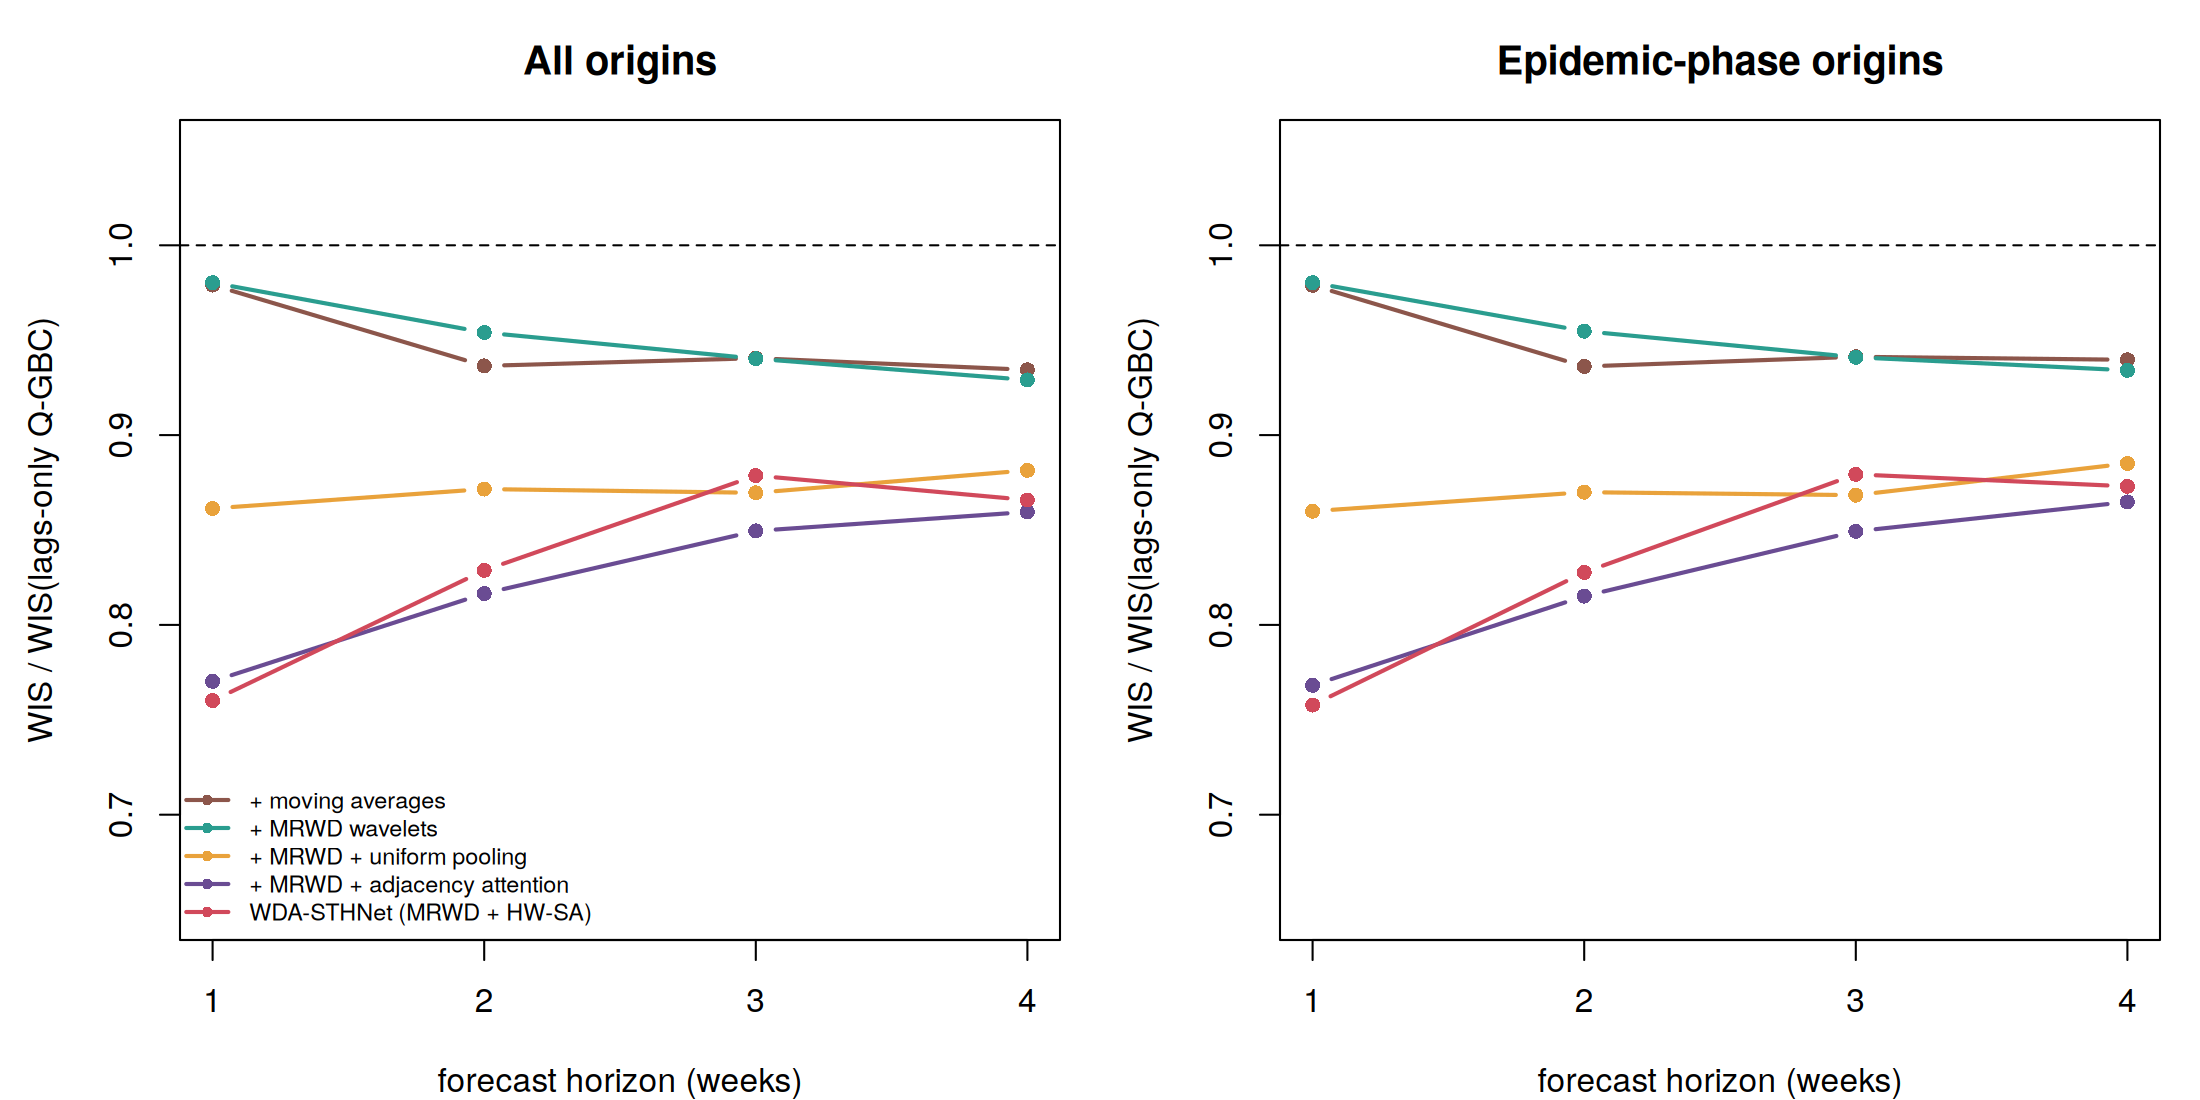
\includegraphics[width=0.98\textwidth]{figures/fig4_ablation.png}\caption{Ablation by horizon: WIS of each variant relative to the lags-only Q-GBC (values below 1 are better). Left: all origins; right: epidemic-phase origins only.}\label{fig:abl}\end{figure}

\subsection{RQ1 --- Wavelets versus moving averages}
Adding the MRWD block to the lags-only booster lowers WIS by \gainWavLags\% (paired difference $-262$, 95\% bootstrap interval $[-324,-202]$, better in 95\% of states; Table~\ref{tab:pair}). Adding trailing moving-average contrasts instead lowers WIS by \gainMALags\%. The direct wavelet-minus-moving-average difference is $+13$ (interval $[-3,32]$; wavelets better in 41\% of states), i.e.\ \textbf{not distinguishable from zero}. Multi-scale smoothing information helps; in this data set the Haar wavelet representation is no better than a few moving-average contrasts. Where the wavelet detail coefficients are used, they are informative: $D^{(2)}$ alone carries 9.1\% of split importance in the final model (Table~\ref{tab:imp}).

\subsection{RQ2 --- Healthcare-weighted spatial attention}
Spatial information is the single most valuable addition: relative to the MRWD-only booster, HW-SA lowers WIS by \gainSpatial\% (paired $-534$, $[-658,-432]$, better in all 37 states). Relative to uniform pooling the gain is \gainUniform\% (interval $[-225,-90]$, better in 86\% of states), so similarity-based, zone-aware weights add value beyond a national average. \textbf{However, the healthcare-access weight does not help:} attention built from adjacency and embedding similarity alone (no $\hc_j$) achieves lower WIS than HW-SA by \lossAdj\% (paired $+54$ for HW-SA, interval $[33,78]$; the adjacency variant is better in 89\% of states). A plausible reading is that $\hc_j$ is a time-invariant scalar that rescales scores for all targets alike, and that its information is already available through $\hc_i$ in the feature vector (it carries only 0.8\% of importance); but our experiment cannot separate this from the possibility that the synthetic generator does not route spread through healthcare capacity. The exploratory state-level pattern in Figure~\ref{fig:gain} is consistent with a modest association between access and skill (correlation of $\hc$ with the WIS ratio to persistence \corrHCrel; with the HW-SA-versus-no-spatial ratio \corrHCwav), but with 37 states and no adjustment for incidence scale we regard it as hypothesis-generating only.

\begin{table}[H]\centering\footnotesize
\resizebox{\textwidth}{!}{\begin{tabular}{lrrrr}
\toprule
Comparison (A vs B) & Mean $\Delta$WIS (A$-$B) & 95\% bootstrap CI & States where A better \\
\midrule
Wavelet vs lags-only & -262 & [-324, -202] & 95\% \\
Wavelet vs moving-average & 13 & [-3, 32] & 41\% \\
HW-SA vs no spatial (wavelet) & -534 & [-658, -432] & 100\% \\
HW-SA vs uniform pooling & -157 & [-225, -90] & 86\% \\
HW-SA vs adjacency attention & 54 & [33, 78] & 11\% \\
WDA-STHNet vs persistence & -9,468 & [-10,911, -8,243] & 100\% \\
\bottomrule
\end{tabular}
}
\caption{Paired comparisons of state-mean WIS (negative = model A better), 37 states.}\label{tab:pair}
\end{table}
\begin{figure}[H]\centering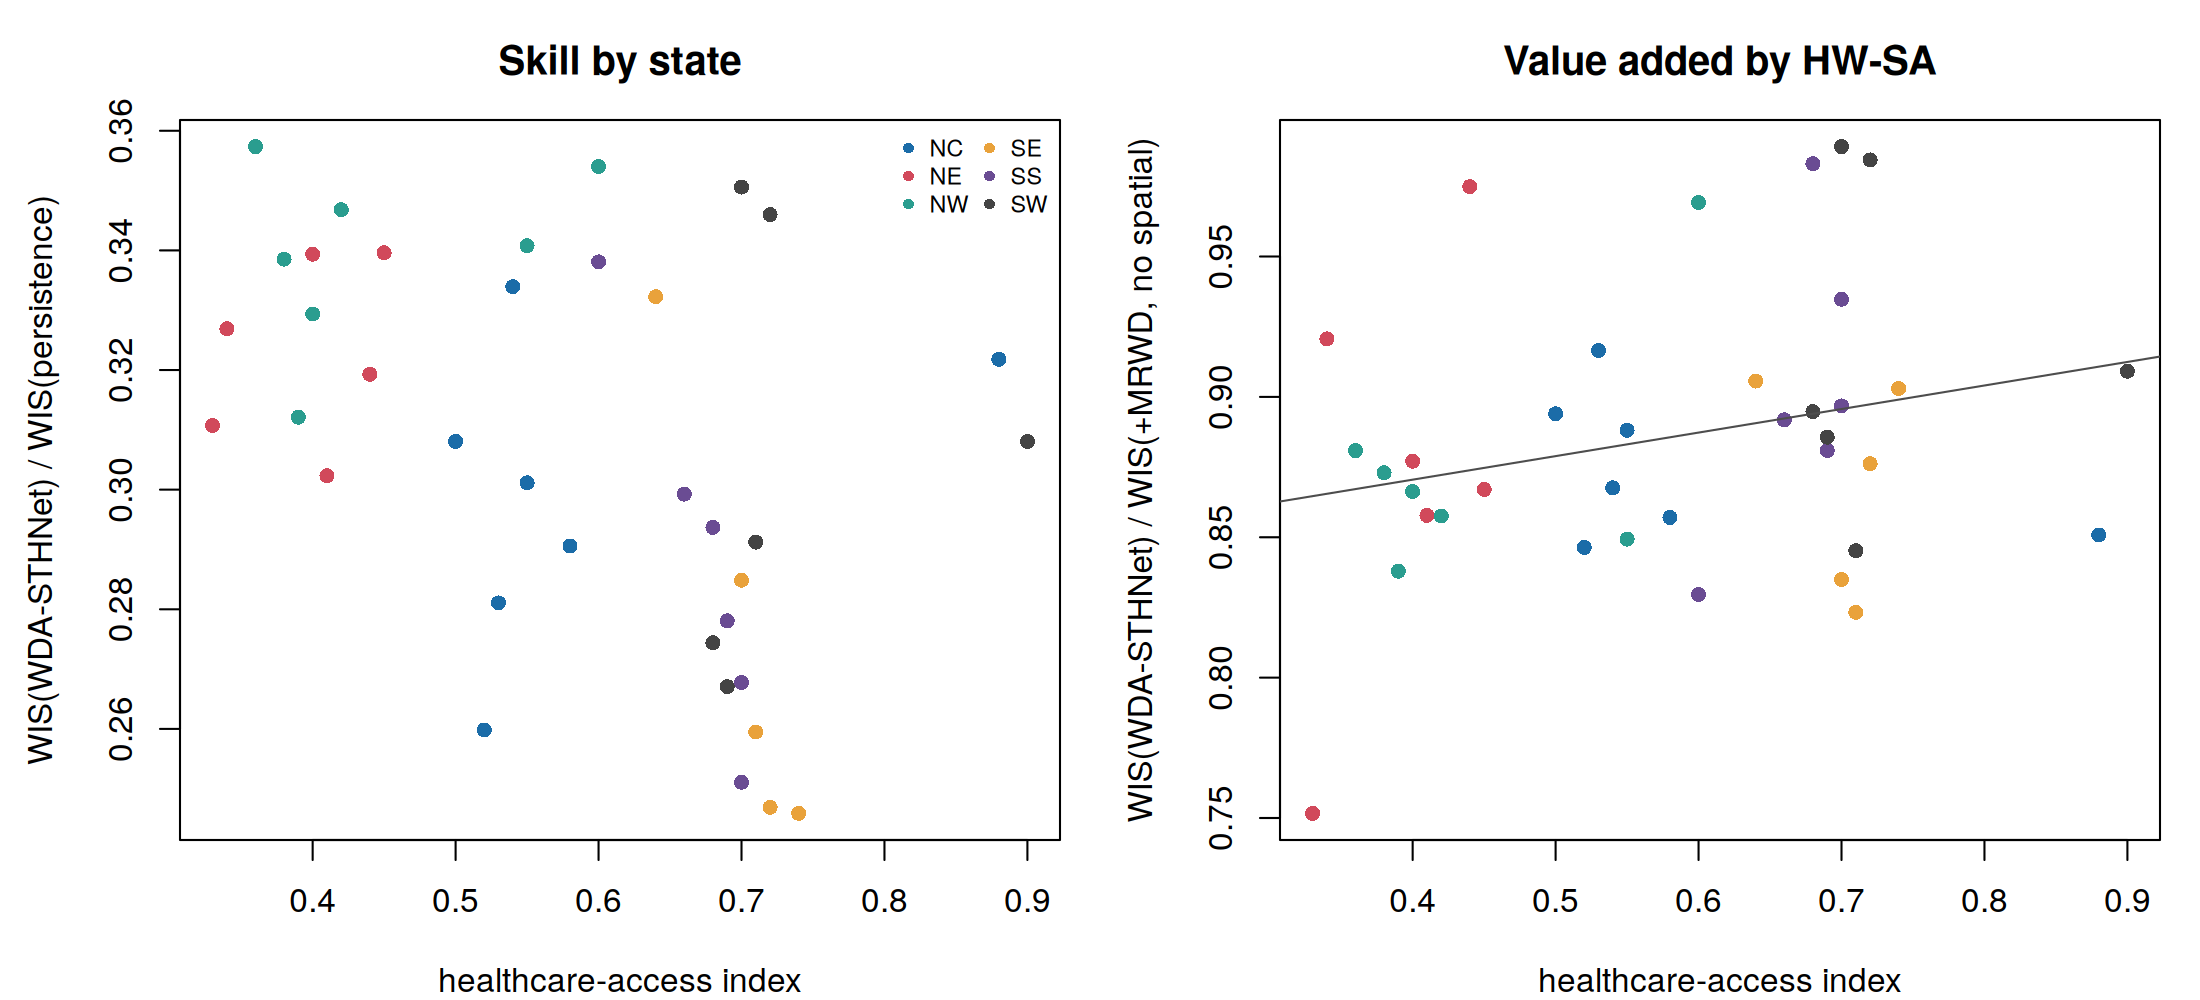
\includegraphics[width=0.98\textwidth]{figures/fig8_state_gain.png}\caption{State-level skill versus healthcare access. Left: WIS ratio of WDA-STHNet to persistence. Right: ratio to the MRWD-only variant (the contribution of HW-SA).}\label{fig:gain}\end{figure}

\subsection{RQ3 --- Calibration across seasons}
Pooled over all forecasts the 90\% interval covers \cvNinety{} of observations and the 50\% interval \cvFifty{} (Table~\ref{tab:main}); both are below nominal, and the 50\% interval is clearly too narrow (the persistence baseline, by construction, is close to nominal in aggregate but with far larger intervals and WIS). Calibration depends on the held-out season (Table~\ref{tab:season}, Figure~\ref{fig:cal}): 90\% coverage is 0.82 in the moderate 2023/24 season, 0.85 in 2025/26 and only 0.70 in the high-severity 2024/25 season, which is also where WIS is highest (6,745 versus 2,788 and 3,083). Coverage declines slowly with horizon (90\%: 0.84 at $h=1$ to 0.75 at $h=4$). The answer to RQ3 is therefore \textbf{no}: quantile boosting trained on two milder seasons does not maintain nominal coverage in a more severe one, which is the expected failure when severity extremes are outside the training range. We did not apply post-hoc recalibration because only two training seasons exist per fold (see Section~\ref{sec:limits}).

\begin{table}[H]\centering\footnotesize
\resizebox{\textwidth}{!}{\begin{tabular}{lrrrrrr}
\toprule
 & \multicolumn{3}{c}{WIS} & \multicolumn{3}{c}{Coverage of 90\% PI} \\
\cmidrule(lr){2-4}\cmidrule(lr){5-7}
Model & 2023/2024 & 2024/2025 & 2025/2026 & 2023/2024 & 2024/2025 & 2025/2026 \\
\midrule
Persistence (empirical growth quantiles) & 9,884 & 18,119 & 13,017 & 0.97 & 0.74 & 0.95 \\
Climatology (week-specific) & 7,889 & 8,891 & 4,743 & 0.65 & 0.32 & 0.91 \\
Q-GBC, lags only & 3,433 & 8,032 & 3,540 & 0.79 & 0.69 & 0.88 \\
Q-GBC + MRWD (Tier 1) & 2,928 & 7,709 & 3,581 & 0.82 & 0.70 & 0.88 \\
\textbf{WDA-STHNet} (MRWD + HW-SA + Q-GBC) & 2,788 & 6,745 & 3,083 & 0.82 & 0.70 & 0.85 \\
\bottomrule
\end{tabular}
}
\caption{WIS and 90\% coverage by held-out season, state level.}\label{tab:season}
\end{table}
\begin{figure}[H]\centering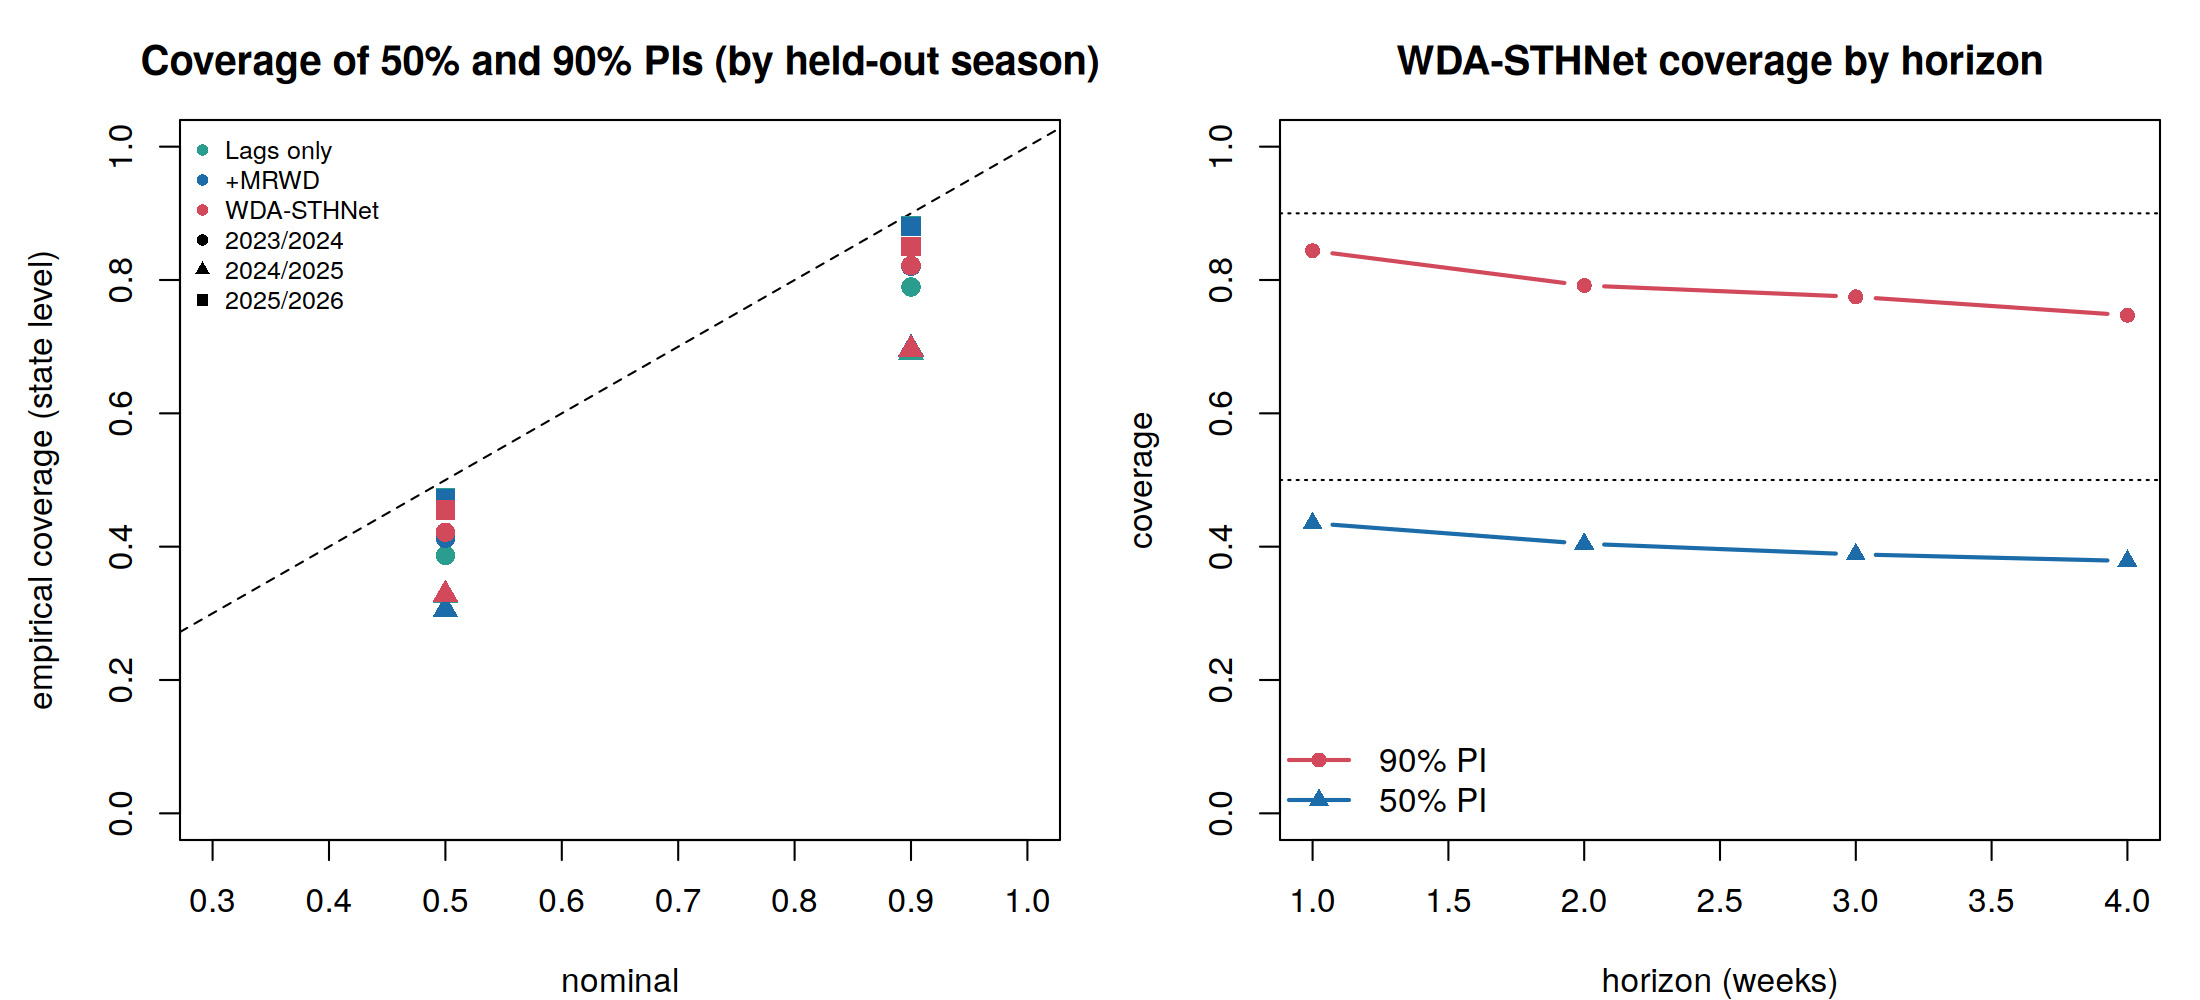
\includegraphics[width=0.98\textwidth]{figures/fig5_calibration.png}\caption{Left: empirical coverage of the 50\% and 90\% intervals by held-out season for three models. Right: coverage of WDA-STHNet by horizon.}\label{fig:cal}\end{figure}

\subsection{National cases, hospitalisations and deaths}
\begin{table}[H]\centering\footnotesize
\resizebox{\textwidth}{!}{\begin{tabular}{llrrrrr}
\toprule
Target & Model & WIS & MAE & RMSE & Cov.\ 50\% & Cov.\ 90\% \\
\midrule
cases & Persistence & 423,821 & 504,650 & 974,969 & 0.50 & 0.89 \\
 & Q-GBC, lags only & 168,717 & 222,001 & 536,731 & 0.43 & 0.79 \\
 & Q-GBC + MRWD & 159,733 & 206,934 & 494,290 & 0.41 & 0.77 \\
 & \textbf{WDA-STHNet} & 157,059 & 202,724 & 485,961 & 0.44 & 0.77 \\
\midrule
hospitalizations & Persistence & 6,279 & 7,709 & 14,811 & 0.49 & 0.89 \\
 & Q-GBC, lags only & 2,287 & 3,005 & 7,801 & 0.42 & 0.75 \\
 & Q-GBC + MRWD & 2,179 & 2,688 & 6,821 & 0.42 & 0.74 \\
 & \textbf{WDA-STHNet} & 2,133 & 2,585 & 6,391 & 0.40 & 0.73 \\
\midrule
deaths & Persistence & 567.2 & 699.3 & 1,318.7 & 0.50 & 0.88 \\
 & Q-GBC, lags only & 221.3 & 285.9 & 684.2 & 0.40 & 0.73 \\
 & Q-GBC + MRWD & 215.8 & 282.3 & 683.2 & 0.41 & 0.72 \\
 & \textbf{WDA-STHNet} & 214.4 & 268.9 & 625.1 & 0.44 & 0.75 \\
\bottomrule
\end{tabular}
}
\caption{National forecasts (LOSO, 43 origins $\times$ 4 horizons $\times$ 3 seasons), count scale.}\label{tab:nat}
\end{table}
For weekly national cases WDA-STHNet attains WIS 157{,}100 against 423{,}800 for persistence (\natGain\% lower) and 168{,}700 for the lags-only booster (6.9\% lower); MAE is 202{,}700 and RMSE 486{,}000. For hospitalisations WIS is 2{,}133 (persistence 6{,}279) and for deaths 214.4 (567.2). The benefit of the wavelet and spatial tiers at national level is smaller and less certain than at state level: only 43 origins per season are available, and the national models have very few training rows. Coverage of the 90\% interval is about 0.77, 0.73 and 0.75 for cases, hospitalisations and deaths. Figure~\ref{fig:fan} shows 1- and 4-week-ahead national forecasts for each held-out season; the peak of the high-severity season is under-predicted at the 4-week horizon.

\begin{figure}[H]\centering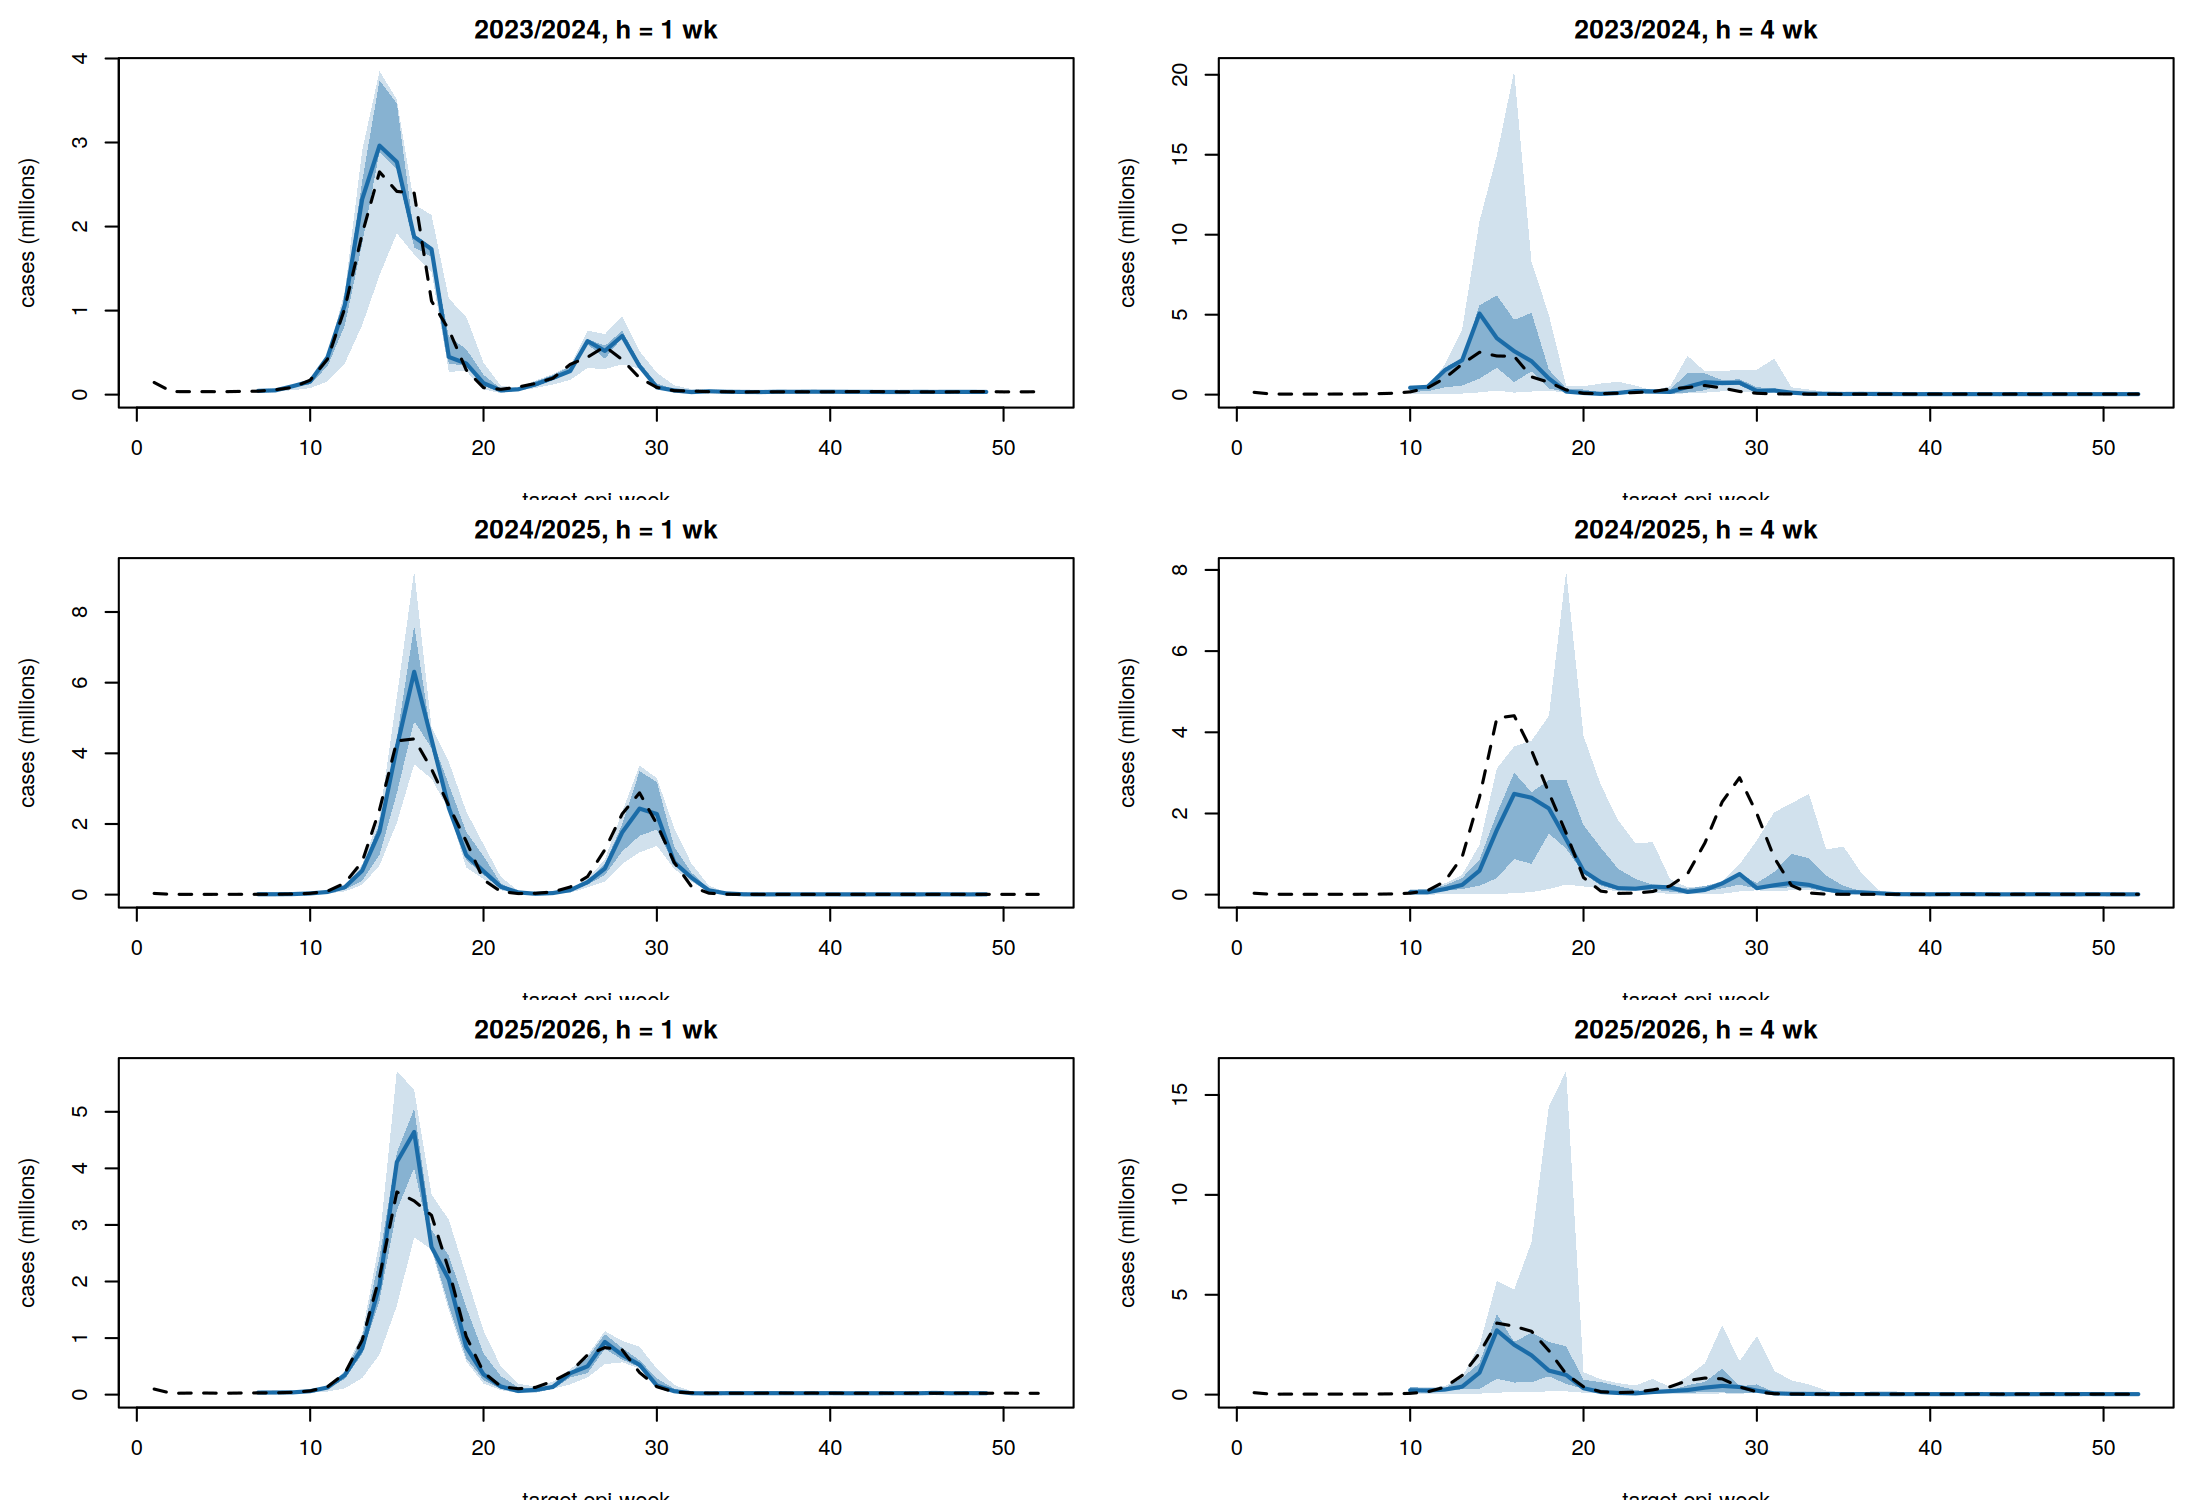
\includegraphics[width=0.98\textwidth]{figures/fig6_national_fan.png}\caption{National WDA-STHNet forecasts of weekly cases with 50\% and 90\% prediction intervals for $h=1$ (left) and $h=4$ (right) in each held-out season; dashed: observed.}\label{fig:fan}\end{figure}
\begin{figure}[H]\centering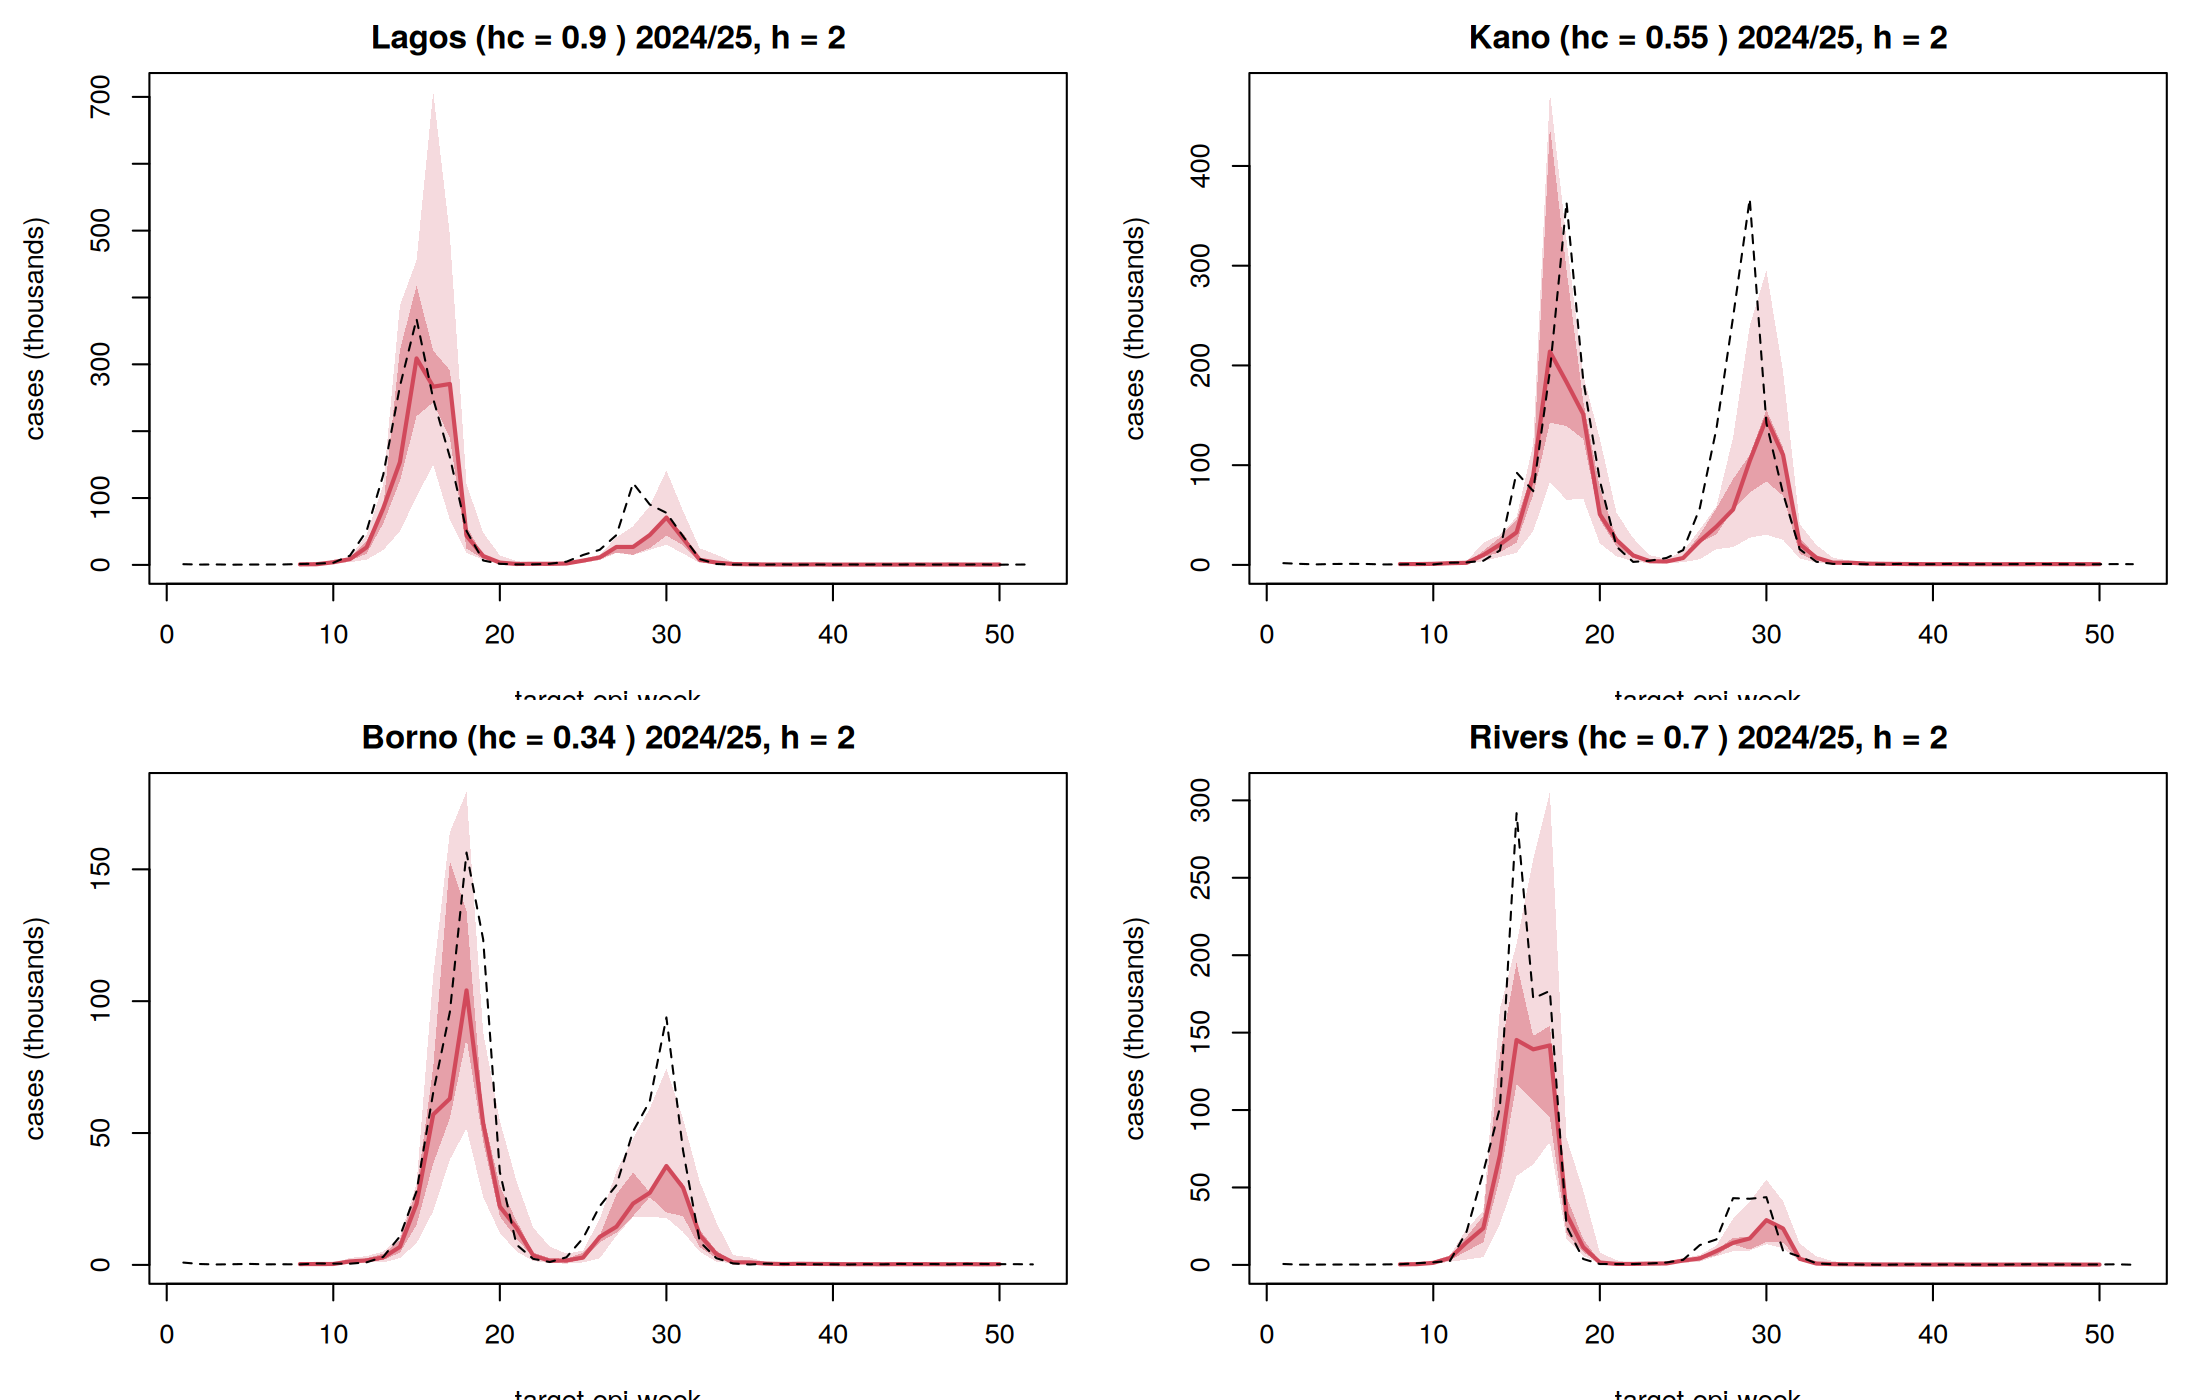
\includegraphics[width=0.98\textwidth]{figures/fig7_state_examples.png}\caption{State-level examples (2024/25, $h=2$): Lagos ($\hc=0.90$), Rivers (0.70), Kano (0.55) and Borno (0.34).}\label{fig:states}\end{figure}

\subsection{Interpretation of the fitted model}
Table~\ref{tab:imp} reports gain-based split importance of the one-week-ahead boosters, summed over the five quantile levels (fold 2025/26 held out). Features from the spatial block account for 27.7\% and the wavelet block for 25.7\% of total importance; the largest single feature is the week-on-week change in neighbour pressure ($\Delta P$, 16.0\%), i.e.\ whether the attention-weighted epidemic in comparable states is accelerating. Importance measures split usage, not causal contribution. Figure~\ref{fig:attn} shows attention matrices at week~14 of 2024/25; HW-SA concentrates weight on same-zone states with similar phase and high access, adjacency-attention likewise but without access, and uniform pooling is flat by construction.
\begin{table}[H]\centering\footnotesize
\resizebox{\textwidth}{!}{\begin{tabular}{llr}
\toprule
Feature & Meaning (group) & Share of importance \\
\midrule
\texttt{sp\_growth} & weekly growth of attention-pooled neighbour pressure (HW-SA (Tier 2)) & 16.0\% \\
\texttt{d2} & 2-week log change (own lags / metadata) & 9.9\% \\
\texttt{wd2} & Haar detail, level 2 (4-wk span) (MRWD (Tier 1)) & 9.1\% \\
\texttt{ex} & excess over early-season baseline (own lags / metadata) & 8.4\% \\
\texttt{d1} & 1-week log change (own lags / metadata) & 7.0\% \\
\texttt{d4} & 4-week log change (own lags / metadata) & 6.8\% \\
\texttt{wd1} & Haar detail, level 1 (2-wk span) (MRWD (Tier 1)) & 6.8\% \\
\texttt{sp\_press} & attention-pooled neighbour pressure (HW-SA (Tier 2)) & 6.2\% \\
\texttt{y} & current log cases (own lags / metadata) & 5.6\% \\
\texttt{sp\_gap} & own incidence minus neighbour pressure (HW-SA (Tier 2)) & 5.5\% \\
\texttt{wsm} & Haar smooth A(3) (MRWD (Tier 1)) & 4.9\% \\
\texttt{wd3} & Haar detail, level 3 (8-wk span) (MRWD (Tier 1)) & 4.9\% \\
\texttt{epi\_week} & epi-week (own lags / metadata) & 3.8\% \\
\texttt{cum} & cumulative incidence (own lags / metadata) & 3.1\% \\
\texttt{hc} & healthcare access (own lags / metadata) & 0.8\% \\
\texttt{sahel} & Sahel flag (own lags / metadata) & 0.7\% \\
\texttt{north} & north flag (own lags / metadata) & 0.3\% \\
\texttt{savanna} & savanna flag (own lags / metadata) & 0.1\% \\
\bottomrule
\end{tabular}
}
\caption{Feature importance of WDA-STHNet ($h=1$, hold-out 2025/26).}\label{tab:imp}
\end{table}
\begin{figure}[H]\centering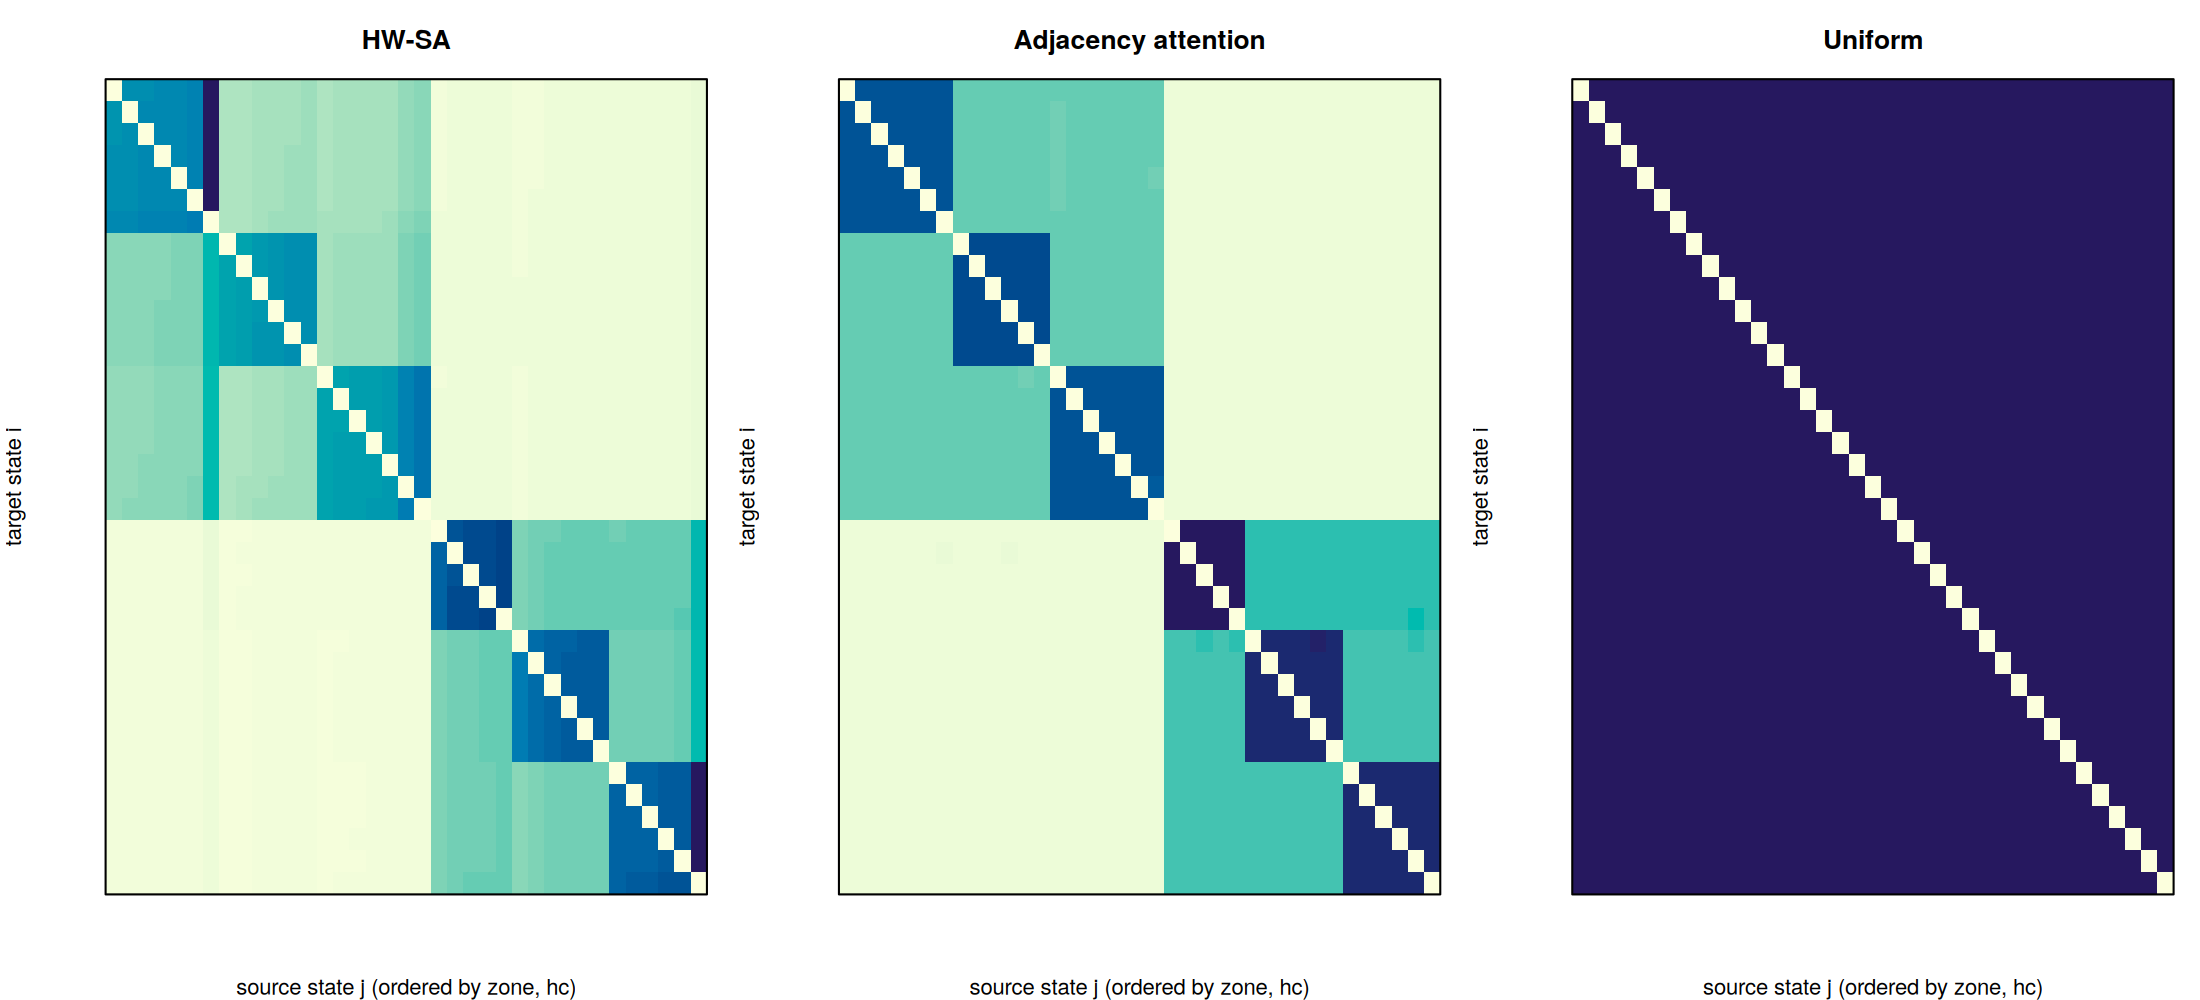
\includegraphics[width=0.98\textwidth]{figures/fig3_attention.png}\caption{Attention weights $\alpha_{ij}$ at epi-week 14 of 2024/25 (rows: target state, columns: source state, ordered by zone and access).}\label{fig:attn}\end{figure}
\begin{figure}[H]\centering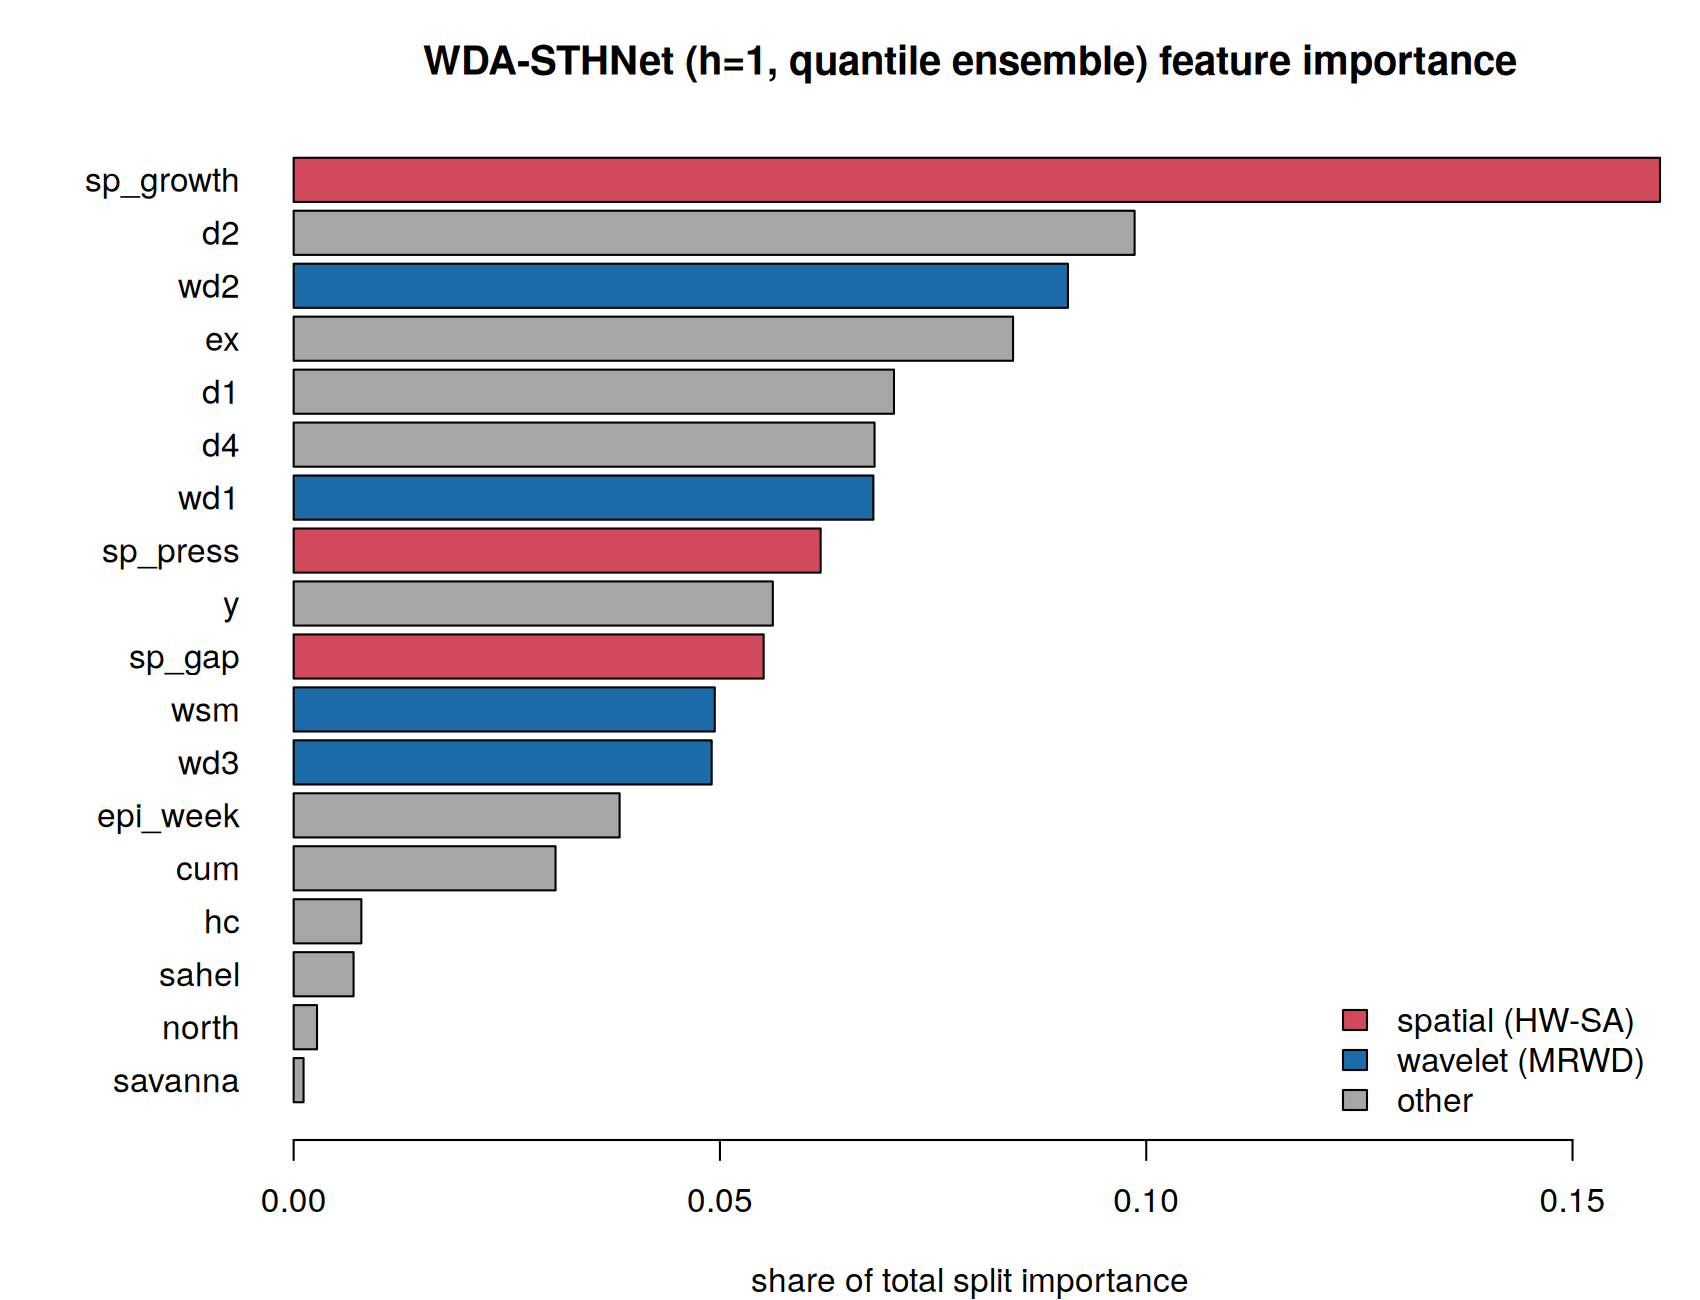
\includegraphics[width=0.75\textwidth]{figures/fig10_importance.png}\caption{Feature importance (share of total split importance).}\label{fig:imp}\end{figure}

%% ------------------------------------------------------------------------
\section{Replication of the Original Script's Protocol}\label{sec:leak}
The original script (i) forms the lags, a three-week rolling mean computed with right alignment (so including the current week), and the Haar smooth and first-level detail of the \emph{same} week; (ii) uses cases of the same week as the response; and (iii) trains on the first 80\% of rows and tests on the last 20\%. Features (i) contain the response: the Haar smooth is $(x_t+x_{t-1})/2$, the detail is $(x_t-x_{t-1})/2$, and the right-aligned mean contains $x_t$. This is a \emph{nowcasting} setting. We reproduced the pipeline with our own Haar transform and Q-GBC (median, 150 trees, depth 4). The test slice is the last 31 weeks (weeks 22--52 of 2025/26, including the Harmattan wave).
\begin{table}[H]\centering\small
\begin{tabular}{lr}
\toprule
Predictor (test: 2025/26, weeks 22--52, $n=31$) & MAE (cases/week) \\
\midrule
Original protocol (same-week features) & 24,421 \\
Same split, same-week features removed & 46,160 \\
Persistence (lag-1) & 51,927 \\
Training-mean predictor & 451,664 \\
\bottomrule
\end{tabular}

\caption{Same-week features versus honest features on the original 80/20 split (median Q-GBC).}\label{tab:leak}
\end{table}
With same-week features the MAE is \origMAE{}; with the same-week features removed it rises to \honestMAE{} (a factor of \origRatio{}), and persistence (lag-1) has MAE \persistMAE{} (Table~\ref{tab:leak}, Figure~\ref{fig:leak}). The 80/20 split on one national series also evaluates one partial season only. We therefore use LOSO with strictly causal features throughout. Reported results of a same-week-feature protocol should not be compared with forecasts at $h\ge1$.
\begin{figure}[H]\centering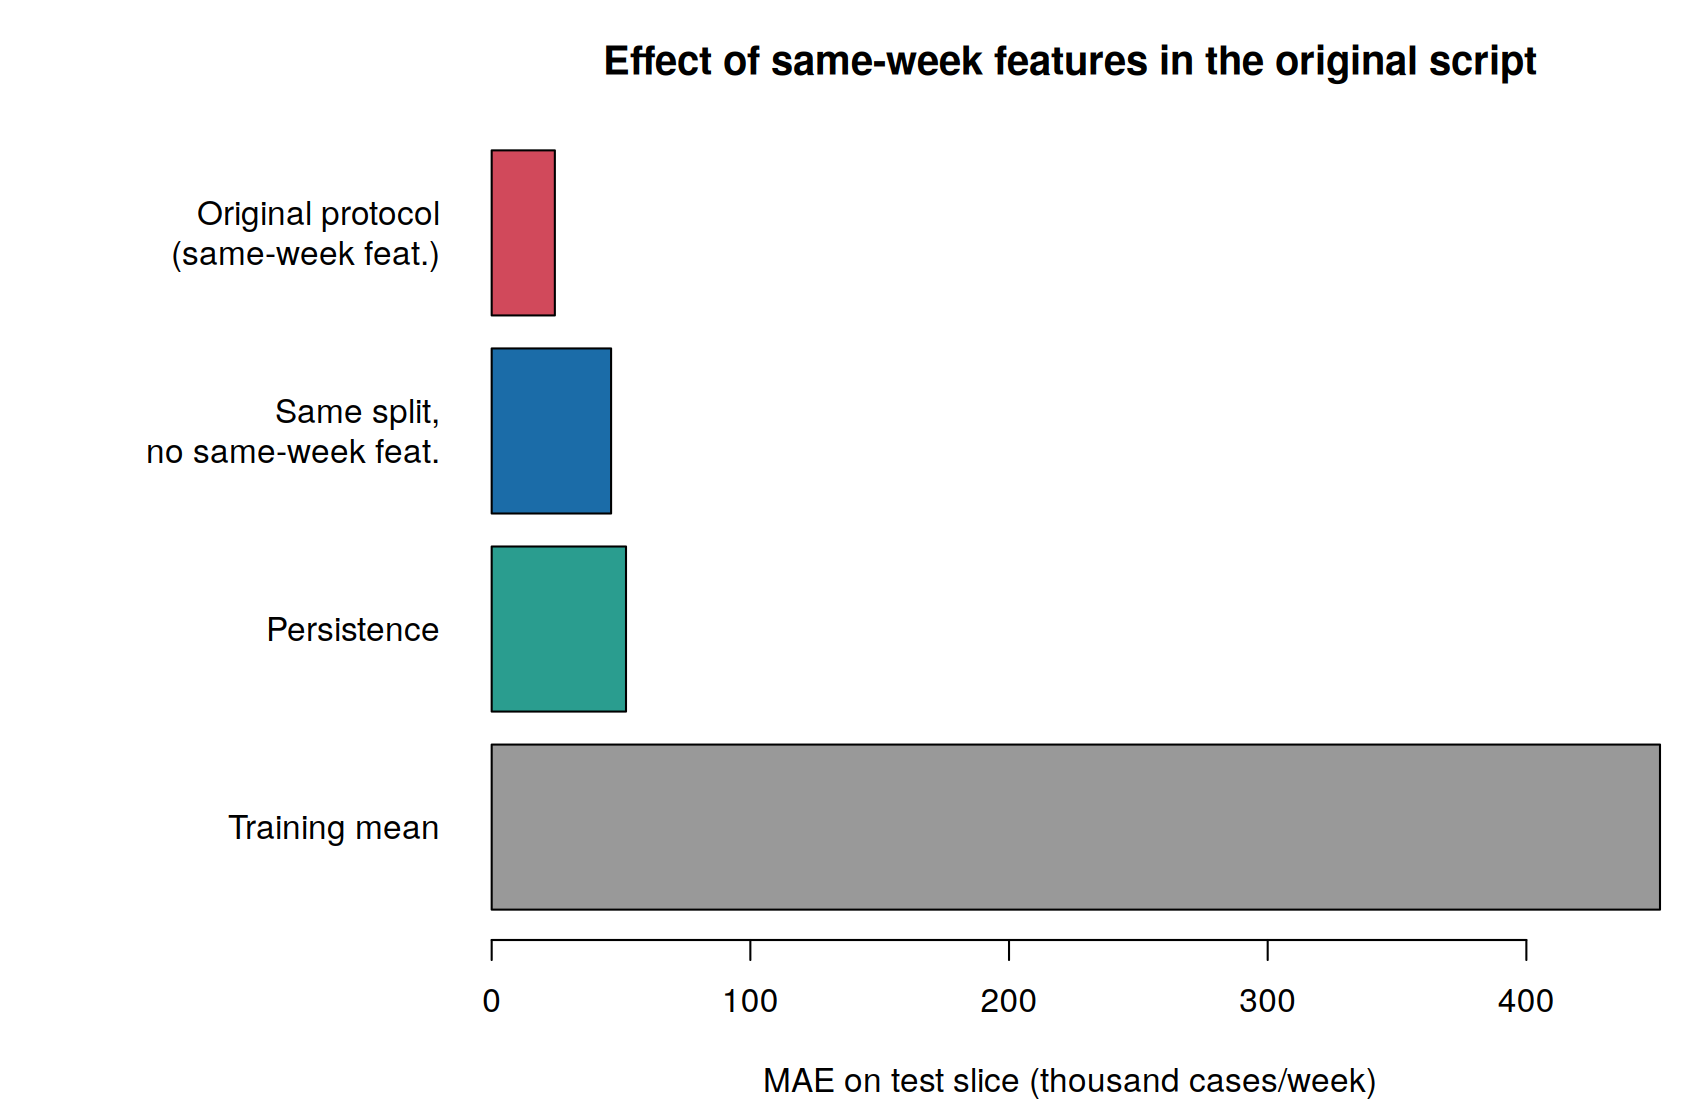
\includegraphics[width=0.7\textwidth]{figures/fig9_leakage.png}\caption{MAE on the original 80/20 test slice with and without same-week features.}\label{fig:leak}\end{figure}

%% ------------------------------------------------------------------------
\section{Policy Implications}
\begin{itemize}
\item \textbf{Short-term surge planning.} In-season 1--4-week-ahead forecasts with the 90\% upper bound (rather than the median) are the appropriate planning quantity for beds, oxygen and antivirals, because intervals are under-dispersed and the high-severity season was under-predicted. Across horizons 1--4, WDA-STHNet's national WIS is about \natGain\% below persistence, which is the practical value of the system.
\item \textbf{Use neighbour pressure as an early-warning indicator.} The strongest predictor is acceleration in the attention-weighted epidemic of comparable states, supporting cross-state surveillance sharing within zones.
\item \textbf{Do not rely on access weighting for forecasting.} Healthcare access remains crucial for \emph{severity} (deaths per hospitalisation), so it should drive resource allocation and mortality-risk communication, but it did not improve forecasts of case counts.
\item \textbf{Recalibrate before operational use.} Coverage of the 90\% interval was 0.70 in the high-severity season; a conformal or severity-conditional widening should be applied once more seasons are available.
\end{itemize}

%% ------------------------------------------------------------------------
\section{Uncertainty, Limitations and Discussion}\label{sec:limits}
\textbf{Sample size.} Only three seasons exist. Each fold trains on two seasons; estimates of the season-to-season effect on coverage rest on three held-out seasons and should be read as indicative. State-level pooling mitigates but does not remove this: state series within a season are strongly dependent through shared weather-driven timing, so the effective number of independent observations is much smaller than the 19{,}092 forecasts per model.\\
\textbf{Averaging.} Count-scale scores are dominated by large states and peak weeks; log-scale scores would weight small states more.\\
\textbf{Spatial prior.} Adjacency is a zone-based proxy, not geography or mobility; the inability of the HW-SA weight to help may reflect this, or the synthetic generator.\\
\textbf{Forecast task.} The model is an in-season forecaster ($h\le4$). It does not produce pre-season forecasts of the next season's peak week, peak size or cumulative burden; those seasonal targets require a different (season-ahead) model, and the quantile-regression approach here does not guarantee coherence between state and national forecasts (the national model is fitted separately).\\
\textbf{Not tuned.} Hyper-parameters ($M=100$, $\nu=0.1$, depth 3) were fixed a priori; no tuning on held-out seasons was performed, which favours honest estimates but may leave accuracy unexploited.\\
\textbf{Originality and components.} The ingredients (Haar MODWT, cosine-similarity attention, quantile boosting, WIS) are established; the contribution is the particular combination (a causal wavelet embedding driving a healthcare-weighted softmax attention that supplies pressure features to a pooled quantile booster) and its verification. Whether this meets the challenge's originality requirement is for the organisers to judge; our ablation shows the part of the architecture contributing most is generic spatial pooling.\\
\textbf{Specification gaps resolved by us:} adjacency definition; embedding definition; use of $\{0.05,\dots,0.95\}$ in place of $\{0.10,\dots,0.90\}$; log-growth targets; removal of same-week features; LOSO instead of an 80/20 split; implementation of Tier~2, which is absent from the original script.

%% ------------------------------------------------------------------------
\section{Conclusions}
We implemented WDA-STHNet end to end and evaluated it without information leakage. It forecasts weekly cases 1--4 weeks ahead much better than persistence (WIS $-\gainVsPersist\%$ at state level, $-\natGain\%$ nationally) and better than a lags-only quantile booster ($-\gainVsLags\%$). Most of the gain over the booster comes from spatial pooling of other states' epidemic momentum (further $-\gainSpatial\%$ beyond wavelet features); wavelet features add \gainWavLags\% but are matched by moving averages; healthcare-weighted attention is slightly worse than attention without the access weight; and prediction intervals are too narrow, particularly in the high-severity season. These findings answer the three research questions in a directly checkable way and give a reproducible baseline against which the more elaborate variants (graph convolution, conformal calibration, season-ahead mechanistic components) can be tested.

\section*{Declaration of AI}
During the preparation of this work, the author used AI assistance (Claude) for code debugging and language refinement. After using this tool, the author reviewed and edited the content as needed and take full responsibility for the content of the report.
\begin{thebibliography}{9}
\bibitem{bracher} Bracher J, Ray EL, Gneiting T, Reich NG (2021). Evaluating epidemic forecasts in an interval format. \emph{PLoS Computational Biology} 17(2): e1008618.
\bibitem{gneiting} Gneiting T, Raftery AE (2007). Strictly proper scoring rules, prediction, and estimation. \emph{J.\ Am.\ Stat.\ Assoc.} 102: 359--378.
\bibitem{percival} Percival DB, Walden AT (2000). \emph{Wavelet Methods for Time Series Analysis}. Cambridge University Press.
\bibitem{friedman} Friedman JH (2001). Greedy function approximation: a gradient boosting machine. \emph{Annals of Statistics} 29: 1189--1232.
\bibitem{koenker} Koenker R, Bassett G (1978). Regression quantiles. \emph{Econometrica} 46: 33--50.
\bibitem{vaswani} Vaswani A, et al.\ (2017). Attention is all you need. \emph{Advances in Neural Information Processing Systems} 30.
\bibitem{therneau} Therneau T, Atkinson B (2023). \emph{rpart: Recursive Partitioning and Regression Trees}. R package.
\bibitem{maepims} MAEPiMS Challenge 2026. \emph{Nigeria Influenza Forecasting Challenge: problem statement and simulated dataset}. The Adejimi Adeniji Foundation.
\bibitem{rcore} R Core Team (2024). \emph{R: A Language and Environment for Statistical Computing}. Vienna.
\end{thebibliography}

%\appendix
%\section{Complete R script}\label{app:code}
%\lstinputlisting{wda_sthnet.R}
%\section{Table-generation script}
%\lstinputlisting{make_tables_tex.R}
\end{document}
